\chapter{Experiments and Results}
\label{chp:6-tests}

\par Every collaborative task previously described was successfully implemented, but in order to validate its quality, performance, and accuracy, we created and performed a series of experiments. They result in quantitative and qualitative metrics and serve as a benchmark of the techniques and tasks developed. After briefly describing the collaborative setup, we outline each test performed on the collaborative tasks and comment on the results. In the end, we also give some remarks on the performance and stability of the overall system.





\section{Collaborative Setup}

% Experimental setup in which the tests were implemented
\par The experimental setup consists on a \ac{ur10e}, with a Weiss Robotics CRG 200 gripper attachment. The vision sensor is a Microsoft Kinect \acs{rgbd} camera and the shared workspace is a simple table, approximately 50cm distant from the robot. The camera is positioned at 2m of height with a \ang{45} downwards orientation and its \ac{fov} is shown in \autoref{fig:kinect}. The complete composition of the setup is shown in \autoref{fig:setup}.

\begin{figure}[h]
    \centering
    \begin{subfigure}{.47\textwidth}
      \centering
      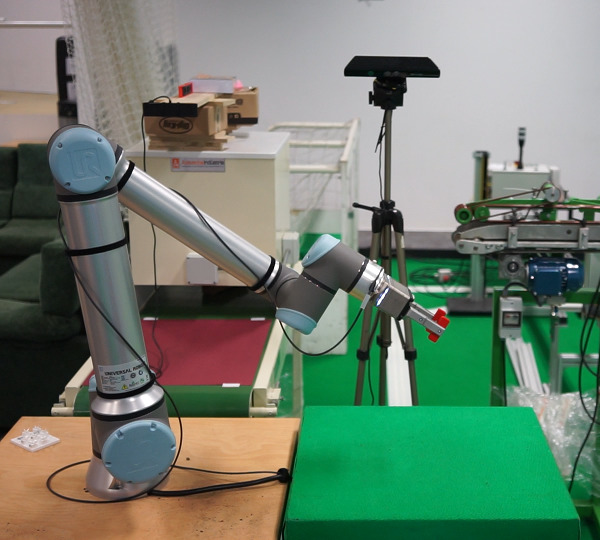
\includegraphics[width=.9\linewidth]{figs/chp6/setup.jpg}
      \caption{Collaborative Setup}
      \label{fig:setup}
    \end{subfigure}%
    \begin{subfigure}{.47\textwidth}
      \centering
      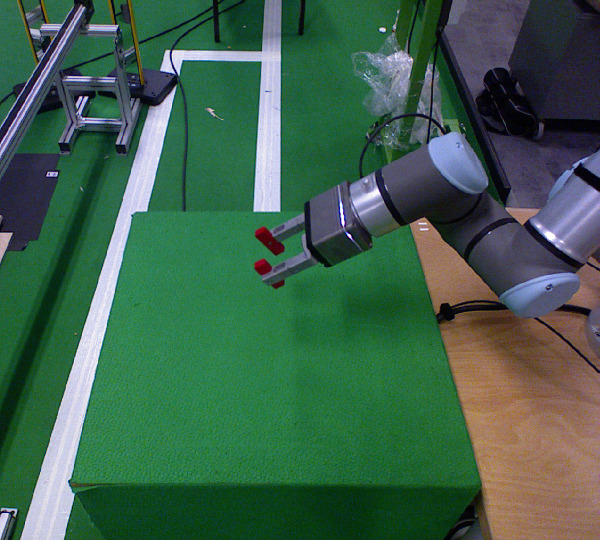
\includegraphics[width=.9\linewidth]{figs/chp6/kinect.jpg}
      \caption{Kinect \ac{fov}}
      \label{fig:kinect}
    \end{subfigure}
    \caption{Views of the experimental shared workspace}
    \label{fig:setup_and_kinect}
\end{figure}





\section{Collaborative Tasks}

% TODO Add introduction to this section

\subsection{Interaction Test}

% Interaction test with 300 taps
\par To validate the use of the \ac{eef} double tap as an interaction interface with the cobot, a test case was developed in which the user would make consecutive double taps in all the directions available and observe if they were correctly registered through the colors of the gripper \acsp{led}. Each direction corresponds to a different color. A double tap interaction is considered a fail when the color of the \acsp{led} does not change, or changes to the wrong color.

\begin{table}[h]
    \centering
    \begin{tabular}{|c|c|c|}
    \hline
    \textbf{Double Taps} & \textbf{Fails} & \textbf{Accuracy} \\ \hline
    300 & 16 & 94,6\% \\ \hline
    \end{tabular}
    \caption{Results of the interaction test}
    \label{tab:interaction_test}
\end{table}

\par In 300 interactions, 94,5\% were correctly registered. Between the fails, the majority were due to weak execution of the double tap. There was record of a few interactions in which the direction was wrongly classified. The cause of this is due to the ambiguous direction in which the user performed the double tap.



\subsection{Hand Guiding}

% Hang Guiding test performed in order to test the payload compensation
\par The accuracy of the \ac{eef} compensation model was already discussed in \autoref{ssec:ft_theory_model}. It has been proved that a force threshold of 2N would be possible since it is higher than the maximum error of the \ac{ft} theoretical model. Despite this fact, it has also been shown in \autoref{ssec:ft_sensor_behavior} that physical interaction with the sensor can cause deviations in its measurements. For this reason, an experimental test was developed to test the accuracy of the compensation model in a real scenario, and the performance of the \ac{hg} task in general.

\begin{figure}[h]
    \centering
    \begin{subfigure}{.2\linewidth}
        \centering
        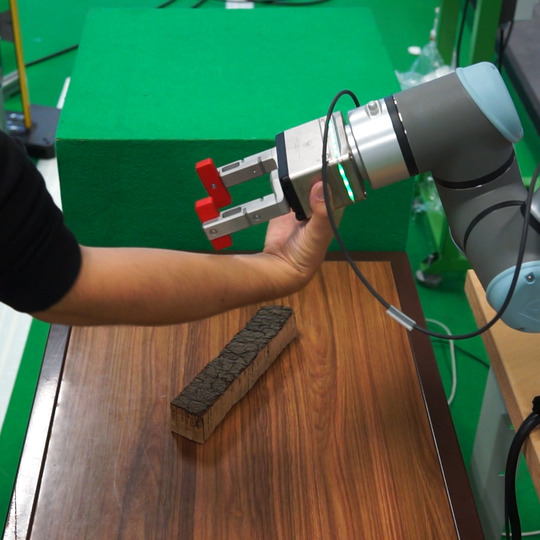
\includegraphics[width=.95\linewidth]{figs/chp6/hg_test_0.jpg}
    \end{subfigure}%
    \begin{subfigure}{.2\linewidth}
        \centering
        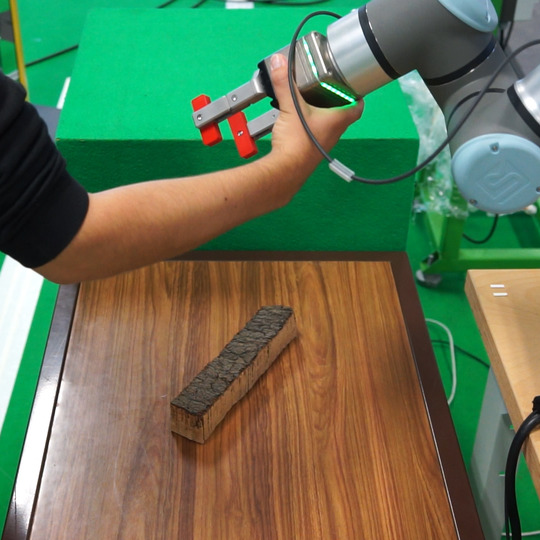
\includegraphics[width=.95\linewidth]{figs/chp6/hg_test_1.jpg}
    \end{subfigure}%
    \begin{subfigure}{.2\linewidth}
        \centering
        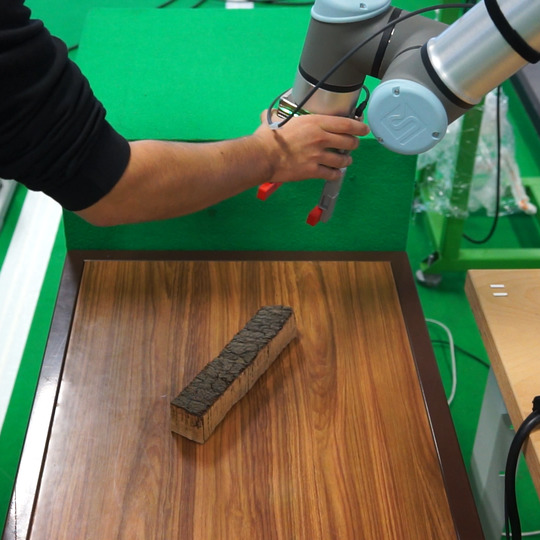
\includegraphics[width=.95\linewidth]{figs/chp6/hg_test_2.jpg}
    \end{subfigure}%
    \begin{subfigure}{.2\linewidth}
        \centering
        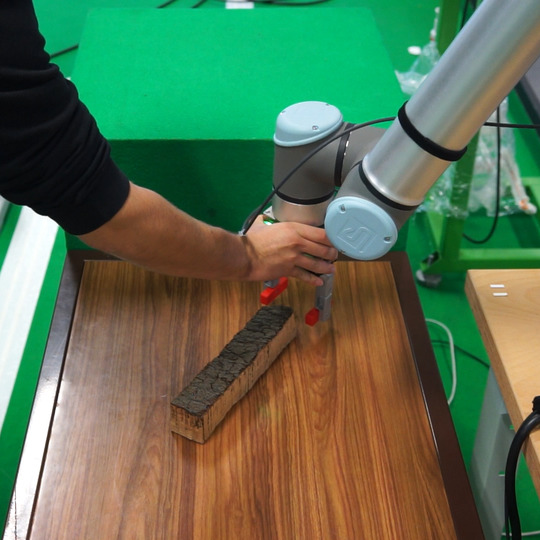
\includegraphics[width=.95\linewidth]{figs/chp6/hg_test_3.jpg}
    \end{subfigure}%
    \begin{subfigure}{.2\linewidth}
        \centering
        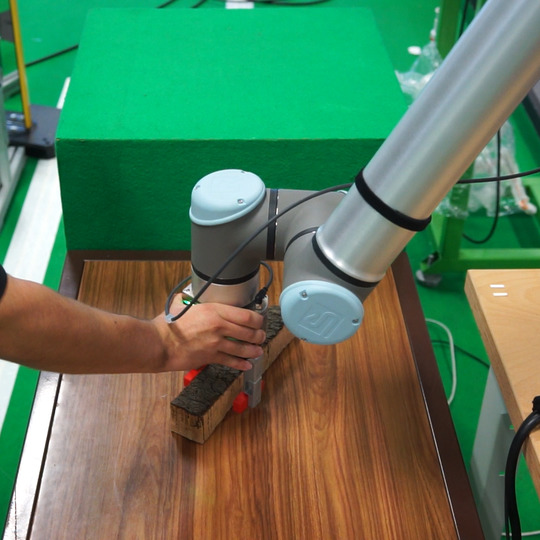
\includegraphics[width=.95\linewidth]{figs/chp6/hg_test_4.jpg}
    \end{subfigure}
    \caption{Succession of steps of the \ac{hg} test}
    \label{fig:hg_test}
\end{figure}

% Description of the hang guiding test
\par The test consists on  \ac{hg} the cobot with the objective of walking the gripper fingers through an object that is placed on the table. The system must compensate the \ac{ft} caused by the gripper in every orientation, therefore the cobot must only move due to external forces caused by the user. On the other hand, the user must align the gripper fingers with the object without difficulty. To test the system responsiveness, the user must walk the gripper through the object in a linear motion, while the gripper finger are aligned with it. The succession of steps for this test is shown in \autoref{fig:hg_test}. 

% Test metrics
\par The metrics for this test are effectiveness and responsiveness. Effective means that the user was able to complete the test, therefore the gripper weight was always correctly compensated and the robot only moved according to the force applied by the user. Responsive means that the robot motion was smooth and specifically in the part that the user must align the gripper fingers with the object on the table, while performing the linear movement, the griper fingers never touched the object. The results should be interpreted as number os successes in the amount of attempts. This test was performed 10 times in multiple settings of force thresholds from the compensation model, and the results are outlined in \autoref{tab:hand_guiding_test}. 

\begin{table}[h]
    \centering
    \begin{tabular}{|c|c|c|c|}
    \hline
    \textbf{\begin{tabular}[c]{@{}c@{}}Force\\ Threshold\end{tabular}} & \textbf{\begin{tabular}[c]{@{}c@{}}Test\\ Effectiveness\end{tabular}} & \textbf{\begin{tabular}[c]{@{}c@{}}Test\\ Responsiveness\end{tabular}} & \textbf{\begin{tabular}[c]{@{}c@{}}Qualitative\\ Performance\end{tabular}} \\ \hline
    \textbf{1N} & 3/10 & 10/10 & Unusable \\ \hline
    \textbf{2N} & 8/10 & 10/10 & Usable \\ \hline
    \textbf{3N} & 10/10 & 10/10 & Balanced \\ \hline
    \textbf{4N} & 10/10 & 9/10 & Satisfactory \\ \hline
    \textbf{5N} & 10/10 & 7/10 & Unresponsive \\ \hline
    \end{tabular}
    \caption{Results of the \ac{hg} performance test}
    \label{tab:hand_guiding_test}
\end{table}

% Interpretation of the results
\par A closer look at the results and an explanation of the qualitative performance will follow:
\begin{itemize}
    \item At 1N of force threshold, the system is unusable. The cobot is mostly moving by itself since the force threshold is too low. This result is expected and serves as a demonstration of the consequences of the inaccuracies of the \ac{ft} sensor.
    \item At 2N, the accuracy results are improved, but not entirely satisfactory. Due to physical interaction with the sensor, there were certain motions that would cause deviations on the \ac{ft} measurements. Despite this fact, with this setting the cobot is very responsive, reacting to very low amounts of force and allowing the gripper to be easily placed exactly where the user wants it to be.
    \item 3N proved to be the best threshold setting. It allowed the correct execution of every test and the loss on responsiveness was not perceptible. With the gripper attachment, 3N will be the default value for force threshold on the \ac{eef} weight compensation model.
    \item 4N and 5N allowed the same accuracy results obtained with 3N but at the cost of motion responsiveness. In short, the user would have to exert higher amounts of force on the \ac{eef} for it to move, causing degradation on its smoothness.
\end{itemize}

% Final remark on the Hang Guiding task
\par The general execution and behavior of the \ac{hg} task is a success. The goal of this test was not only to find the best system parameters to obtain the best possible behavior, but also to prove that the orchestration of \ac{ros} nodes and the algorithms they implement, proposed in this dissertation, is well founded and effective.



\subsection{Object Manipulation}

% Requirements for the object manipulation task
\par The object manipulation task requires the dynamic attachment of extra weight to the cobot \ac{eef}. It has been showed previously that the \ac{eef} weight compensation model supports dynamic changing of the weight and \ac{cog} parameters, but the performance of this manipulation task is directly proportional to the accurate measurement of this parameters.

% Weight measurement test
\par The first test regarding this task should be to find both system and \ac{ft} sensor performance on correctly measuring the weight of the coupled object. In order to do this, a 1Kg iron weight will be gripped by the cobot 10 times in 6 different orientations. These orientations consist on vertically aligning each \ac{ft} axis, in each direction, with gravity, in order to obtain the accuracy of each measurement component, and can be seen in \autoref{fig:weight_poses}.

\begin{figure}[h]
    \centering
    \begin{subfigure}{.166\linewidth}
        \centering
        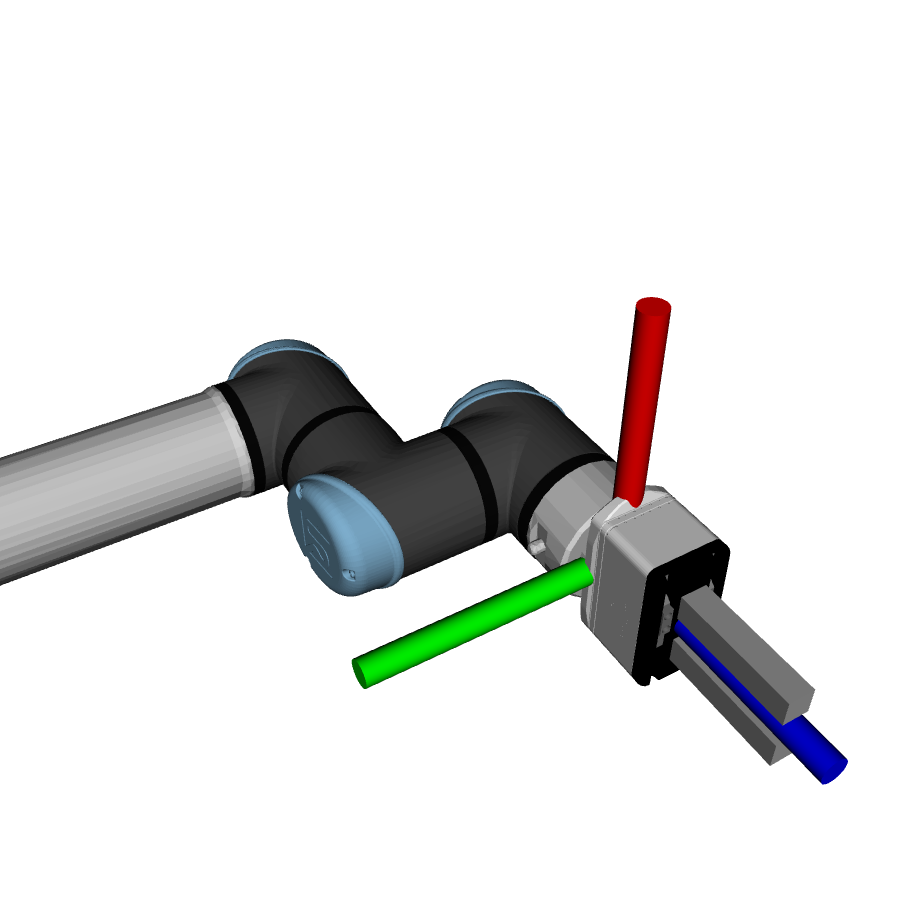
\includegraphics[width=\linewidth]{figs/chp6/weight_x_pos.png}
    \end{subfigure}%
    \begin{subfigure}{.166\linewidth}
        \centering
        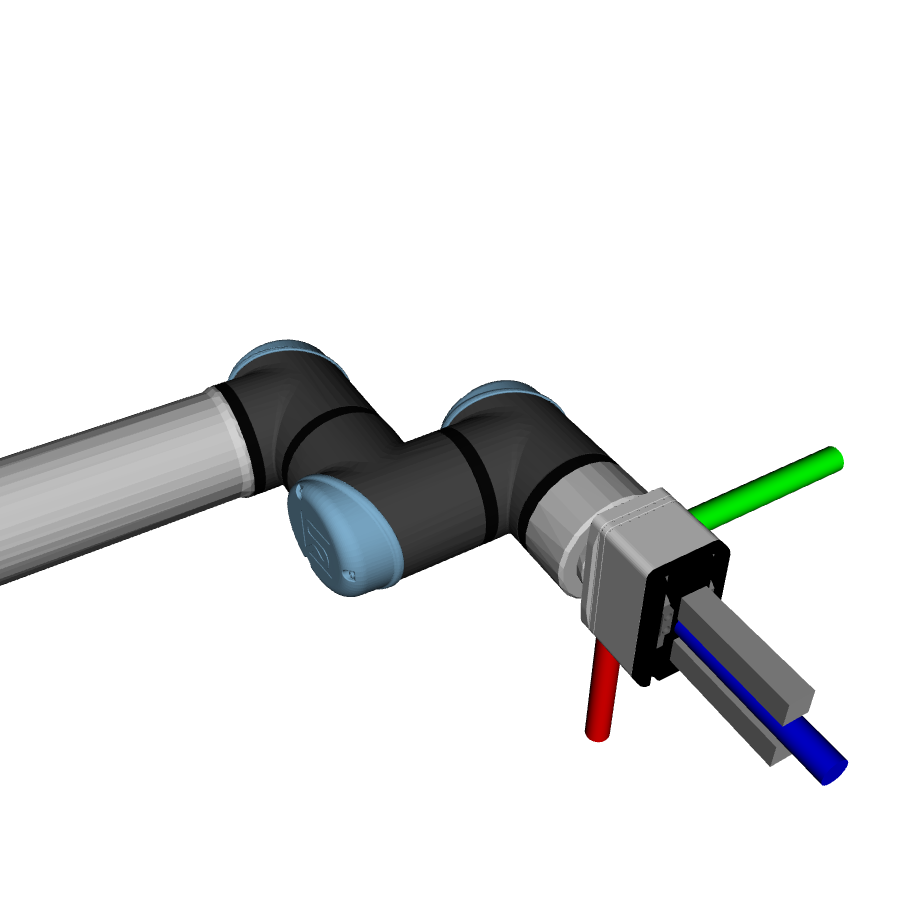
\includegraphics[width=\linewidth]{figs/chp6/weight_x_neg.png}
    \end{subfigure}%
    \begin{subfigure}{.166\linewidth}
        \centering
        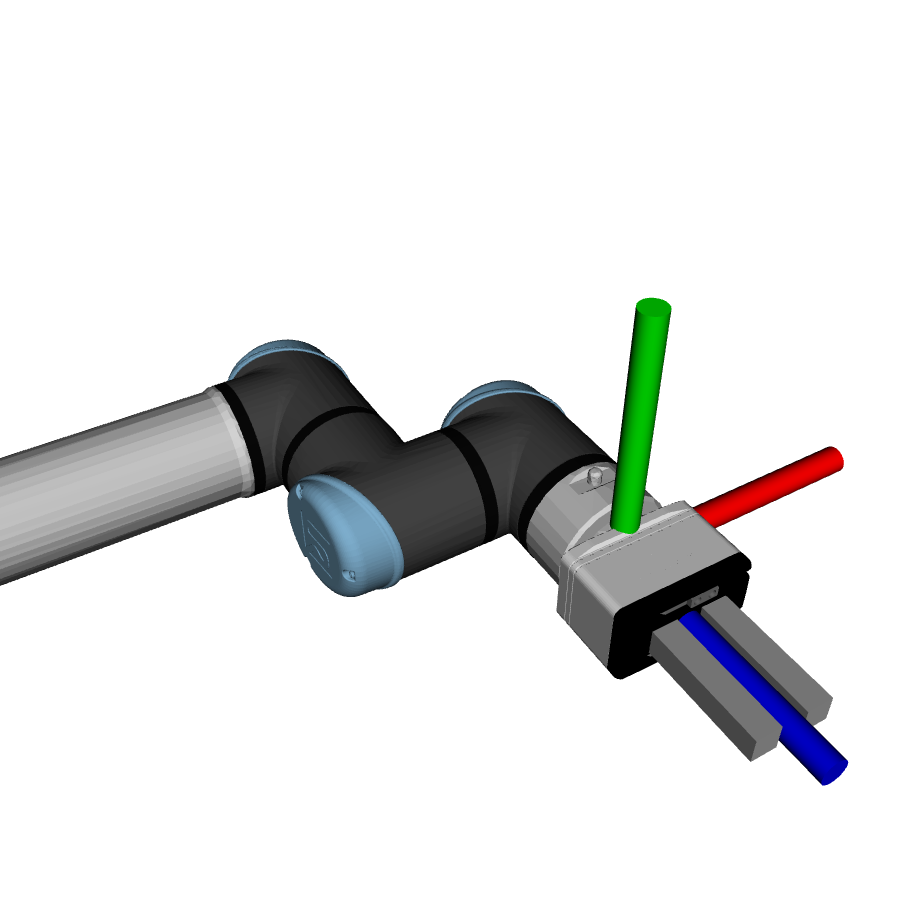
\includegraphics[width=\linewidth]{figs/chp6/weight_y_pos.png}
    \end{subfigure}%
    \begin{subfigure}{.166\linewidth}
        \centering
        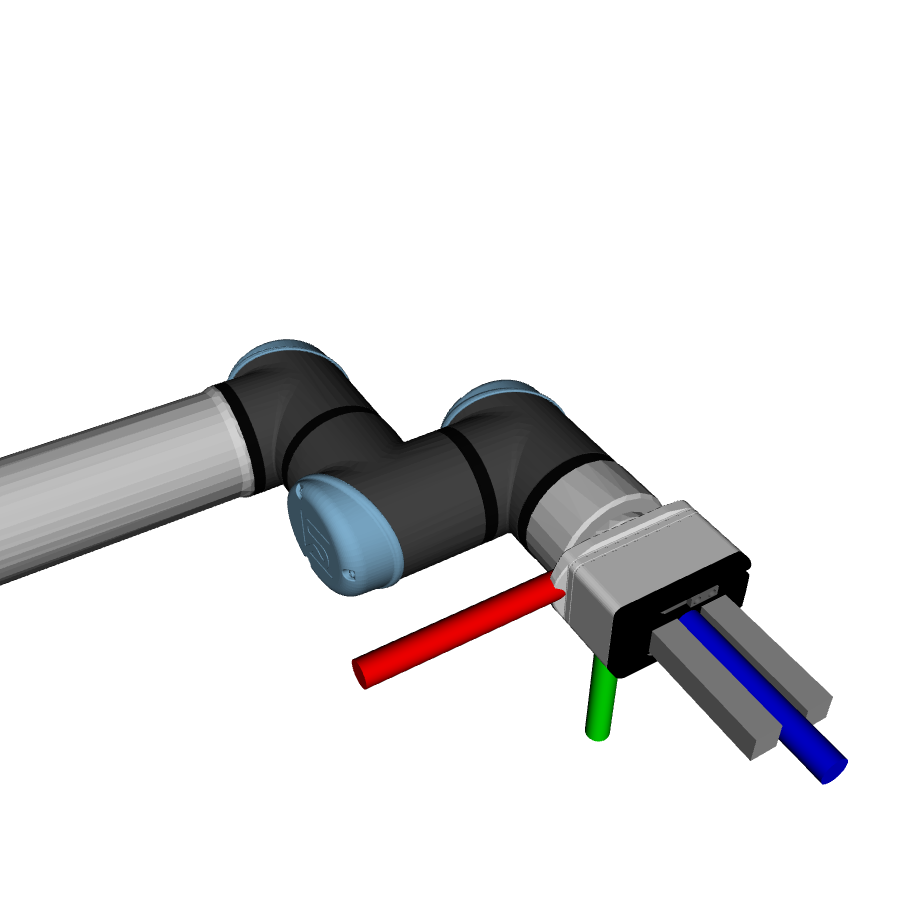
\includegraphics[width=\linewidth]{figs/chp6/weight_y_neg.png}
    \end{subfigure}%
    \begin{subfigure}{.166\linewidth}
        \centering
        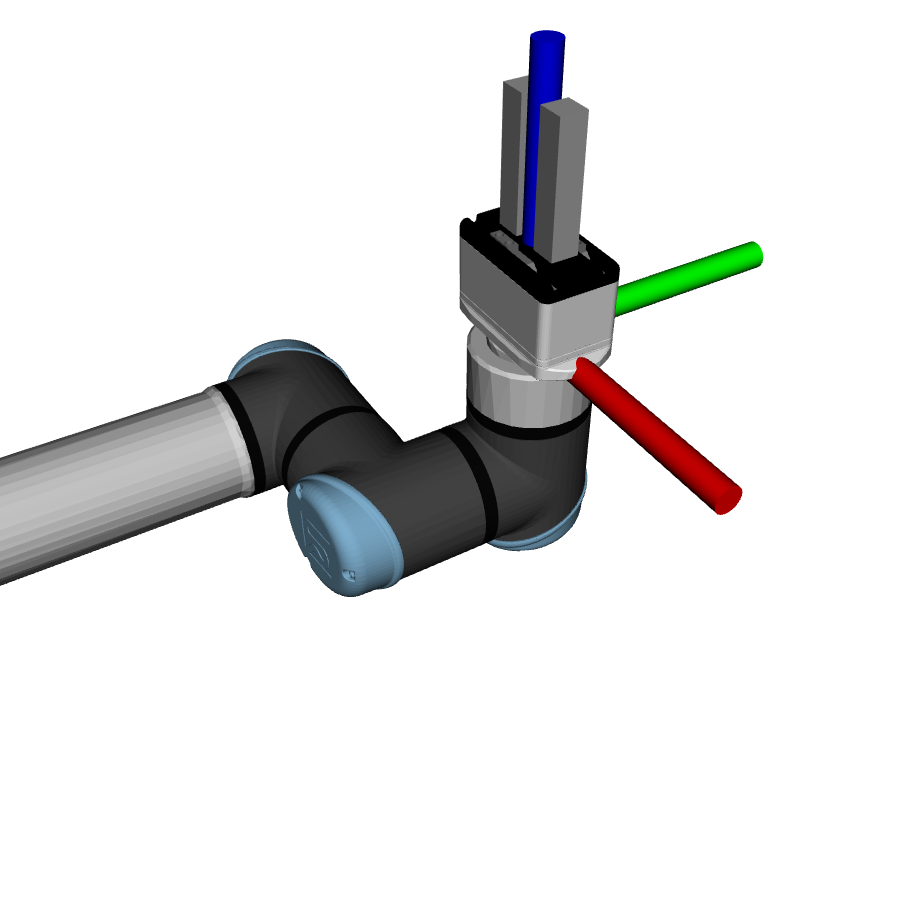
\includegraphics[width=\linewidth]{figs/chp6/weight_z_pos.png}
    \end{subfigure}%
    \begin{subfigure}{.166\linewidth}
        \centering
        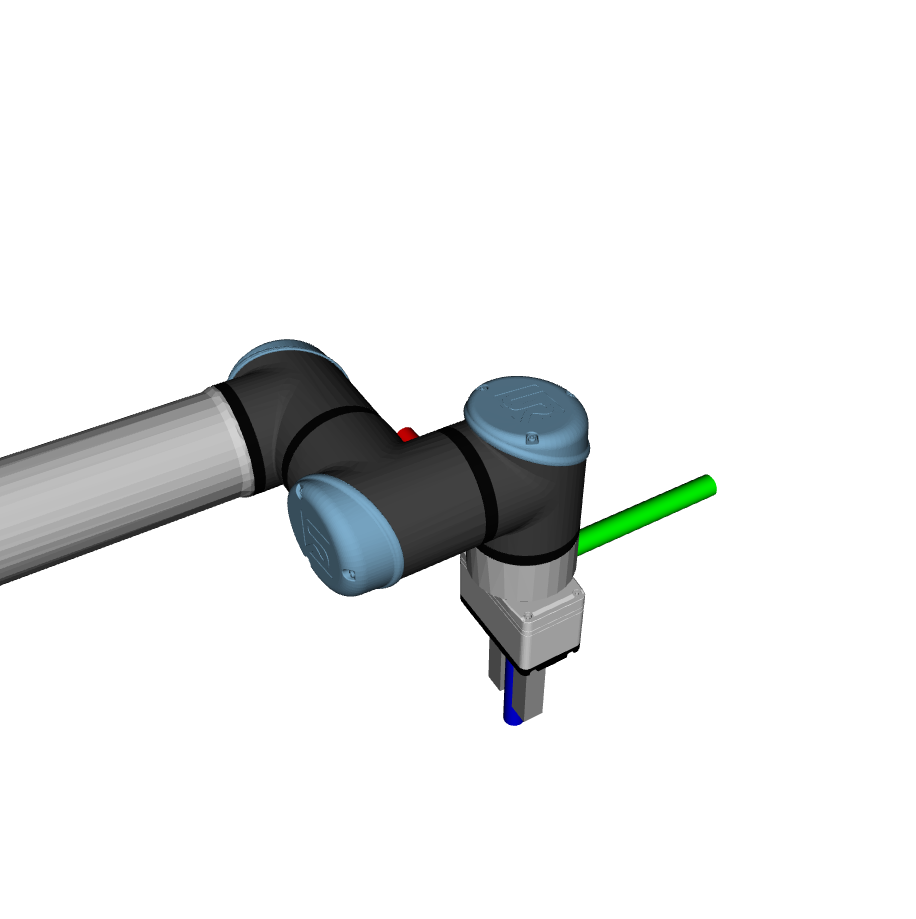
\includegraphics[width=\linewidth]{figs/chp6/weight_z_neg.png}
    \end{subfigure}
    \caption{6 different \ac{eef} weight measurement poses}
    \label{fig:weight_poses}
\end{figure}

% Outline of the measurements in 6 graphs
\par The raw results are outlined in \autoref{fig:weight_result}. As it is evidently seen, changing the measuring axis has a significant effect on the reported measured weight.

\begin{figure}[h]
    \centering
    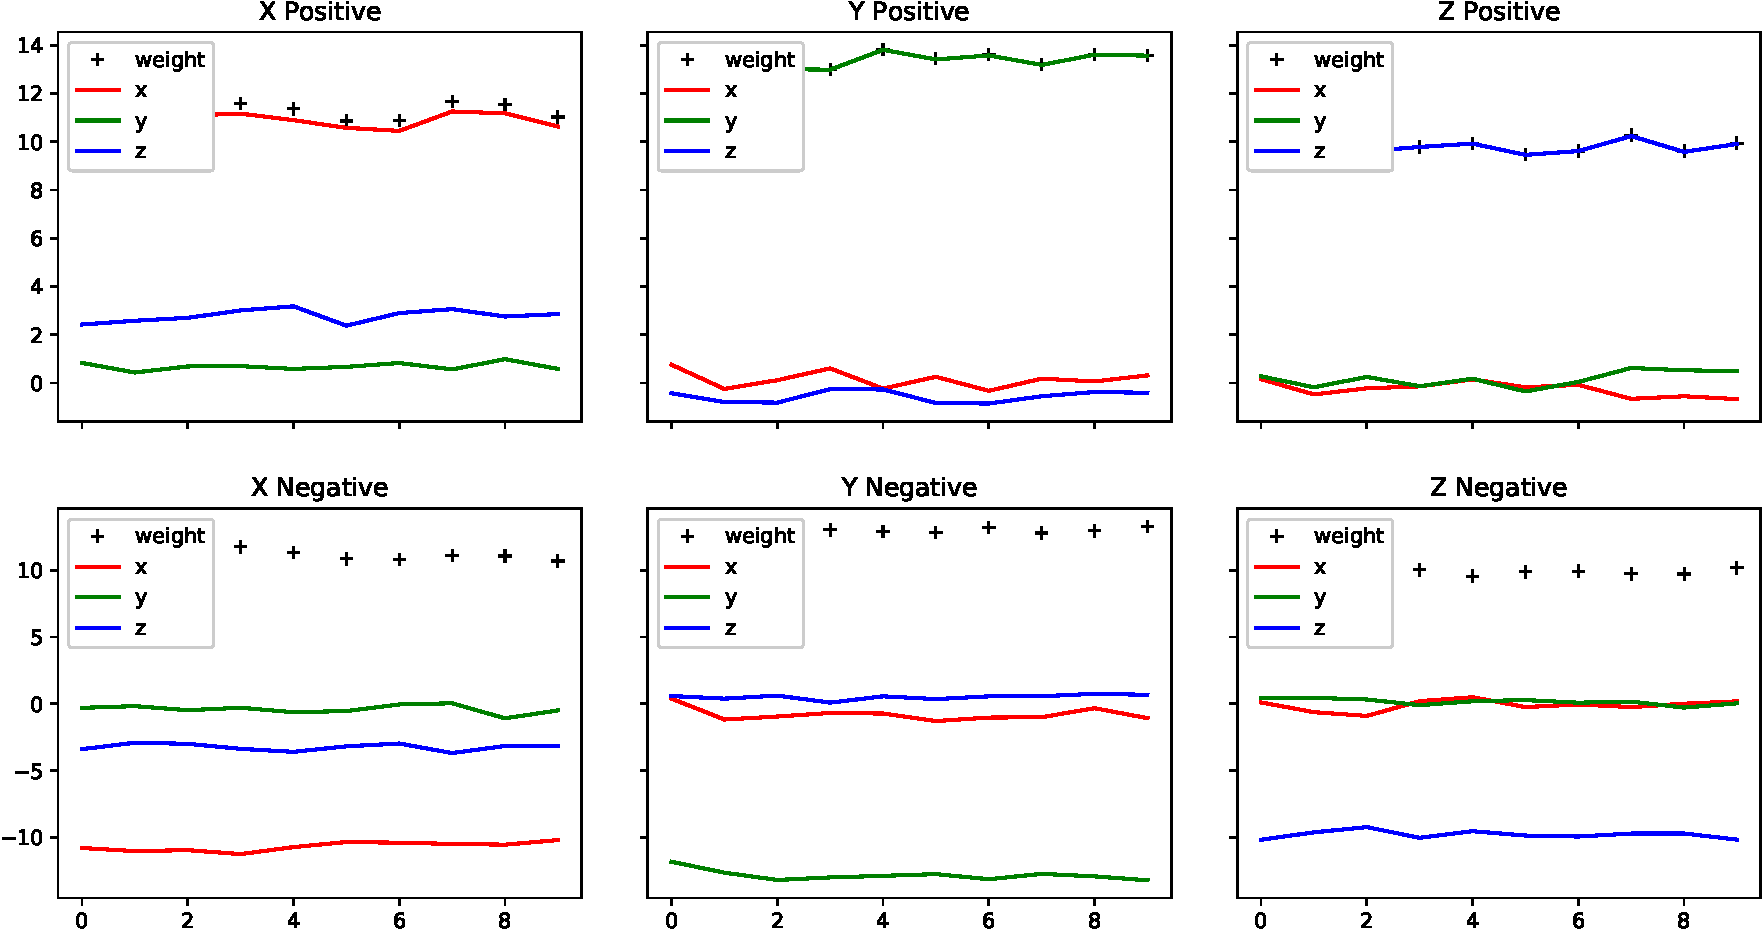
\includegraphics[width=0.8\linewidth]{figs/chp6/weight_measurements.pdf}
    \caption{Results of the weight measurement test in each position}
    \label{fig:weight_result}
\end{figure}

% Results in table view with DLS correction and Scalar correction
\par \autoref{tbl:weight_results} gives a closer look at the some statistics from the weight measurement tests. All values are to be read as weight in Kg.

\begin{table}[h]
    \centering
    \begin{tabular}{|l|c|c|c|}
    \hline
    \multicolumn{1}{|c|}{\textbf{\begin{tabular}[c]{@{}c@{}}Weight Test\end{tabular}}} & \textbf{Raw} & \textbf{\begin{tabular}[c]{@{}c@{}}\ac{dls}\\ Correction\end{tabular}} & \textbf{\begin{tabular}[c]{@{}c@{}}Scalar \\ Correction\end{tabular}} \\ \hline
    \textbf{X Positive} & 1.144 & 1.210 & 1.001 \\ \hline
    \textbf{X Negative} & 1.138 & 1.209 & 1.008 \\ \hline
    \textbf{Y Positive} & 1.369 & 1.229 & 1.025 \\ \hline
    \textbf{Y Negative} & 1.311 & 1.176 & 0.982 \\ \hline
    \textbf{Z Positive} & 0.992 & 1.219 & 1.016 \\ \hline
    \textbf{Z Negative} & 0.999 & 1.229 & 1.024 \\ \hline \hline
    \textbf{Average} & 1.159 & 1.213 & 1.011 \\ \hline
    \textbf{Std Dev} & 0.146 & 0.038 & 0.031 \\ \hline
    \end{tabular}
    \caption{Detailed results and statistics from the weight measurement tests}
    \label{tbl:weight_results}
\end{table}

% Interpretation of the results and explanation of DLS and Scalar corrections
\par At first, the raw values are neither precise nor accurate showing a wrong weight average and an arguably high standard deviation. Applying the correction constants obtained from \ac{dls} optimization in \autoref{ssec:ft_theory_model}, it is possible to improve the precision of the measurements, with a significantly lower standard deviation, but the final average weight value is still far from the correct. Applying a scalar correction with the value of 1.2 provides an accurate and precise weight measurement, with an improved and much lower standard deviation, meaning it is expected that in real use scenarios, the weight of a coupled object should only deviate, in the maximum, by this value.

% Object manipulation test
\par Assuming the weight is correctly obtained, a real time test was performed to demonstrate that the \ac{eef} weight compensation model can sustain the same levels of accuracy independent of the weight coupled to the robot. \autoref{fig:object_result} shows a real time test where Wrist1 and Wrist2 joints are rotated causing multiple \ac{eef} orientations. Similar to previous real time tests the \ac{eef} weight is compensated with minimal error.

\begin{figure}[h]
    \centering
    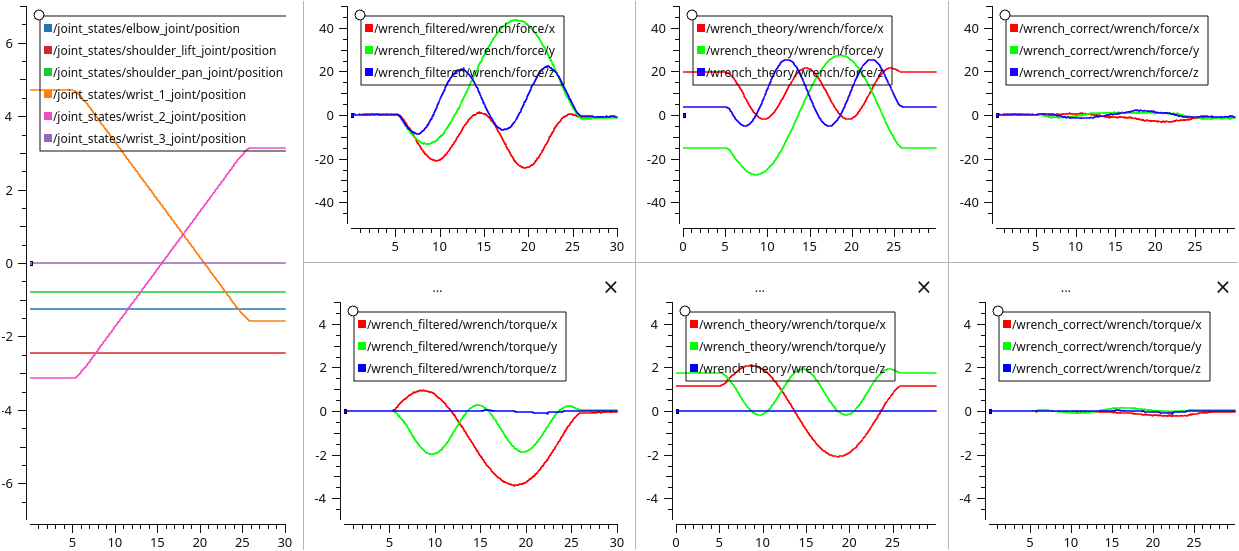
\includegraphics[width=0.9\linewidth]{figs/chp6/object_result.png}
    \caption{Result of the compensation architecture applied in a real time test}
    \label{fig:object_result}
\end{figure}

\begin{figure}[h]
    \centering
    \begin{subfigure}{.2\linewidth}
        \centering
        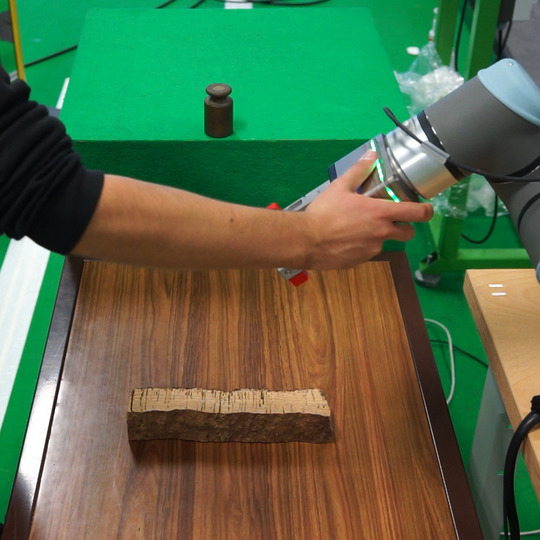
\includegraphics[width=.95\linewidth]{figs/chp6/om_test_0.jpg}
    \end{subfigure}%
    \begin{subfigure}{.2\linewidth}
        \centering
        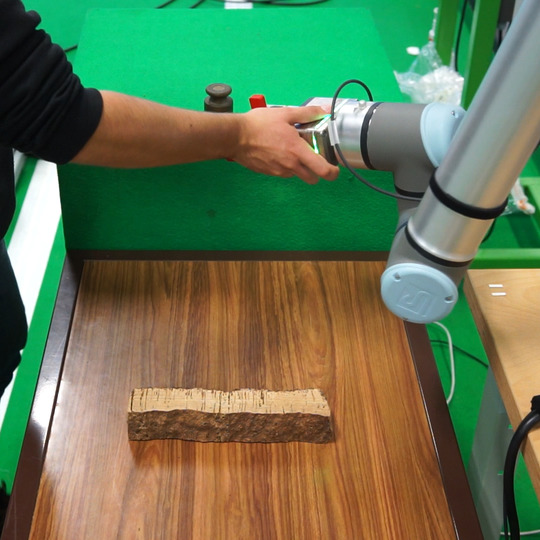
\includegraphics[width=.95\linewidth]{figs/chp6/om_test_1.jpg}
    \end{subfigure}%
    \begin{subfigure}{.2\linewidth}
        \centering
        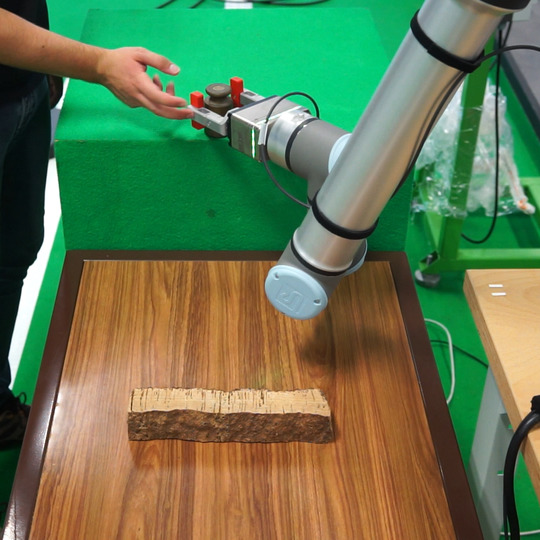
\includegraphics[width=.95\linewidth]{figs/chp6/om_test_2.jpg}
    \end{subfigure}%
    \begin{subfigure}{.2\linewidth}
        \centering
        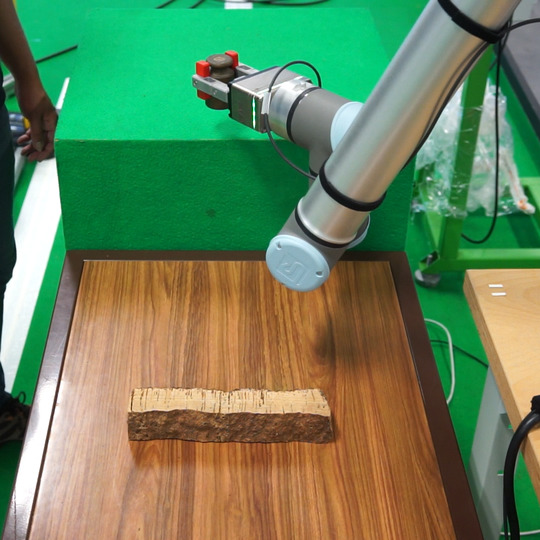
\includegraphics[width=.95\linewidth]{figs/chp6/om_test_3.jpg}
    \end{subfigure}%
    \begin{subfigure}{.2\linewidth}
        \centering
        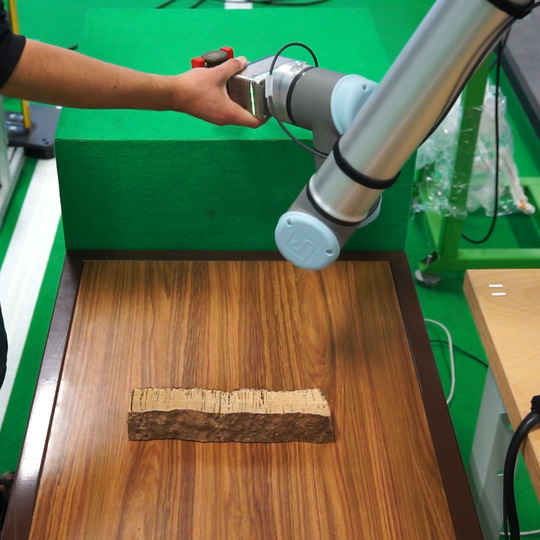
\includegraphics[width=.95\linewidth]{figs/chp6/om_test_4.jpg}
    \end{subfigure}
    \par\smallskip
    \begin{subfigure}{.2\linewidth}
        \centering
        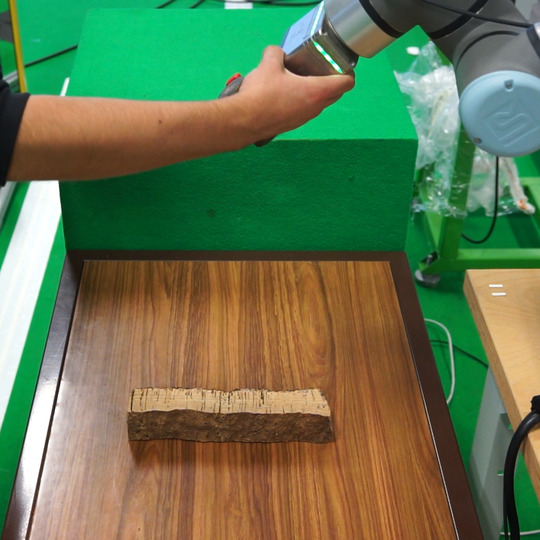
\includegraphics[width=.95\linewidth]{figs/chp6/om_test_5.jpg}
    \end{subfigure}%
    \begin{subfigure}{.2\linewidth}
        \centering
        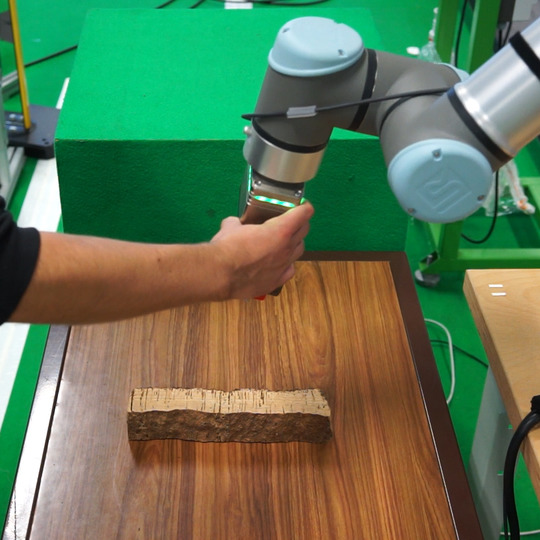
\includegraphics[width=.95\linewidth]{figs/chp6/om_test_6.jpg}
    \end{subfigure}%
    \begin{subfigure}{.2\linewidth}
        \centering
        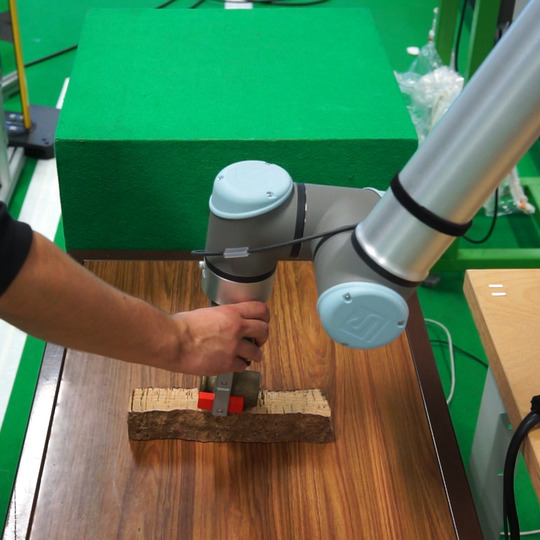
\includegraphics[width=.95\linewidth]{figs/chp6/om_test_7.jpg}
    \end{subfigure}%
    \begin{subfigure}{.2\linewidth}
        \centering
        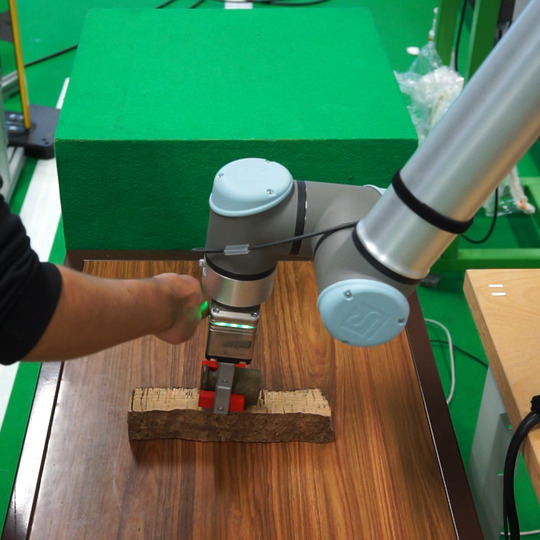
\includegraphics[width=.95\linewidth]{figs/chp6/om_test_8.jpg}
    \end{subfigure}%
    \begin{subfigure}{.2\linewidth}
        \centering
        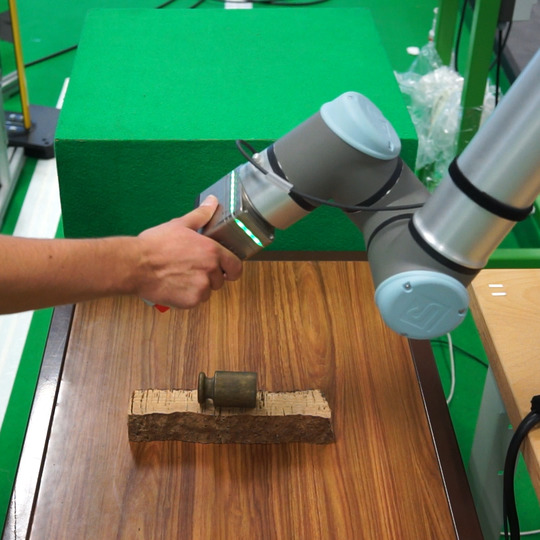
\includegraphics[width=.95\linewidth]{figs/chp6/om_test_9.jpg}
    \end{subfigure}
    \caption{Succession of steps of the object manipulation test}
    \label{fig:om_test}
\end{figure}

% Explanation of the test that was performed
\par For the same reasons as in the \ac{hg} tests, weight compensation error is not enough to validate this task. Furthermore, since extra weight is added, it is suspected that the deviations caused by physical interaction with the \ac{ft} sensor will increase compared to the previous task. This time, the collaborative test consists on \ac{hg} the cobot, aligning it with a stationary object in the environment, give the order to grip it, wait for the system to calibrate its payload and manipulate the object with both linear and angular movements, in order to release it at another location in the environment. \autoref{fig:om_test} shows the succession of steps in this test. The evaluation metrics are the same as in th \ac{hg} test, and it was also repeated 10 times in each force threshold setting.

\begin{table}[h]
    \centering
    \begin{tabular}{|c|c|c|c|}
    \hline
    \textbf{\begin{tabular}[c]{@{}c@{}}Compensation\\ Accuracy\end{tabular}} & \textbf{\begin{tabular}[c]{@{}c@{}}Test\\ Effectiveness\end{tabular}} & \textbf{\begin{tabular}[c]{@{}c@{}}Test\\ Responsiveness\end{tabular}} & \textbf{\begin{tabular}[c]{@{}c@{}}Qualitative\\ Performance\end{tabular}} \\ \hline
    \textbf{1N} & 0/10 & 10/10 & Unusable \\ \hline
    \textbf{2N} & 3/10 & 10/10 & Unusable \\ \hline
    \textbf{3N} & 7/10 & 10/10 & Usable \\ \hline
    \textbf{4N} & 10/10 & 8/10 & Satisfactory \\ \hline
    \textbf{5N} & 10/10 & 5/10 & Unresponsive \\ \hline
    \end{tabular}
    \caption{Results of the object manipulation performance test}
    \label{tab:object_manipulation_test}
\end{table}

% Interpretation of the results
\par \autoref{tab:object_manipulation_test} presents the results of the test and similar to the previous task a qualitative interpretation of them will follow: 
\begin{itemize}
    \item Similar to the \ac{hg} task and for the same reasons, 1N of force threshold is unusable.
    \item At 2N, the results improve but there is still prone to a lot of deviations, therefore not enough.
    \item 3N show enough improvements on the results to be considered usable, since the majority of tests are completed. Given this fact, in a real manipulation scenario, the objective would be for the robot to never fail, even if it means sacrificing on responsiveness.
    \item 4N would be the ideal force threshold value for this task since it allows the completion of all the tests without significant sacrifice on motion responsiveness.
    \item 5N presents results similar to the \ac{hg} task where all tests are completed at the cost of motion smoothness.
\end{itemize}

% Necessity of increasing the force threshold based on payload weight
\par In order for these tests to be successfully completed, the value of force threshold of the weight compensation model needed to be increased. This is caused by 2 factors: 

\begin{itemize}
    \item Increasing the \ac{eef} coupled weight increases the inaccuracies of the \ac{ft} sensor due to interaction with the user, as explained in \autoref{chp:3-ft-sensor-correction}.
    \item The generation of force values from the theoretical \ac{ft} model is directly impacted by the configured value of object weight, which is measured and set in real time, when the robot grabs the object. Inaccuracies on weight measurement due to incorrect handover, or simply due to the arguably weak force accuracy specification value of 5.5N, can directly impact the performance of the theoretical model, whose ultimate goal is to model the behavior of the real \ac{ft} sensor.
\end{itemize}

\par The solution to this problem seems to rely on adapting the force threshold value of the theoretical \ac{ft} model according to the current payload weight. With a 1.5Kg gripper tool, 3N of force threshold meant manipulating the tool with a 1:5 force to motion ratio. Gripping a 1Kg iron weight, and increasing the force threshold to 5N allows to maintain the same ratio and be able to successfully and accurately manipulate the conjoint weight. The loss on responsiveness is an acceptable tradeoff for the fact that, in the end, the tests in question were effectively completed. 

% TODO Review this section linguistically



\subsection{Collision Free Execution of an Industrial Task}
\label{sec:colision_tests}

\par The validity of the collision avoidance architecture has already been shown in \autoref{sec:obstacle-architecture}, and the execution of an industrial task is a simple succession of predefined steps. To obtain performance metrics on this task and the collision avoidance architecture, a series of tests will be performed, both in simulation and in a real environment, and its results outlined.


\subsubsection{Gazebo Simulator Environment}

\par The first test consists on a trajectory between two poses and a sphere obstacle strategically placed on top of the trajectory. Detailed parameters of this test are outlined in \autoref{tbl:obstacle_test}, where position is to read as XYZ coordinates in meters, and orientation as XYZ rotation in degrees (\textdegree).

\begin{table}[h]
    \centering
    \begin{tabular}{|c|c|c|lccc}
    \cline{1-3} \cline{5-7}
    \textbf{Trajectory} & \textbf{Position} & \textbf{Orientation} & \multicolumn{1}{l|}{} & \multicolumn{1}{c|}{\textbf{Obstacle}} & \multicolumn{1}{c|}{\textbf{Position}} & \multicolumn{1}{c|}{\textbf{Radius}} \\ \cline{1-3} \cline{5-7} 
    \textbf{Start} & (1.0, 0.0, 0.4) & (0, 90, 90) & \multicolumn{1}{l|}{} & \multicolumn{1}{c|}{\textbf{Sphere}} & \multicolumn{1}{c|}{(0.8, 0.8, 0.35)} & \multicolumn{1}{c|}{0.1} \\ \cline{1-3} \cline{5-7} 
    \textbf{End} & (0.0, 1.0, 0.4) & (0, 90, 90) &  & \multicolumn{1}{l}{} & \multicolumn{1}{l}{} & \multicolumn{1}{l}{} \\ \cline{1-3}
    \end{tabular}
    \caption{Parameters for the base obstacle avoidance test}
    \label{tbl:obstacle_test}
\end{table}

\par This test was created and executed in the Gazebo simulator. The offline trajectory was obtained with the \ac{rrt} Connect planner, that is implemented on the \ac{ompl}. Visual representation of the environment and trajectory is shown in \autoref{fig:obstacle_test}.

\begin{figure}[h]
    \centering
    \begin{subfigure}{.5\linewidth}
        \centering
        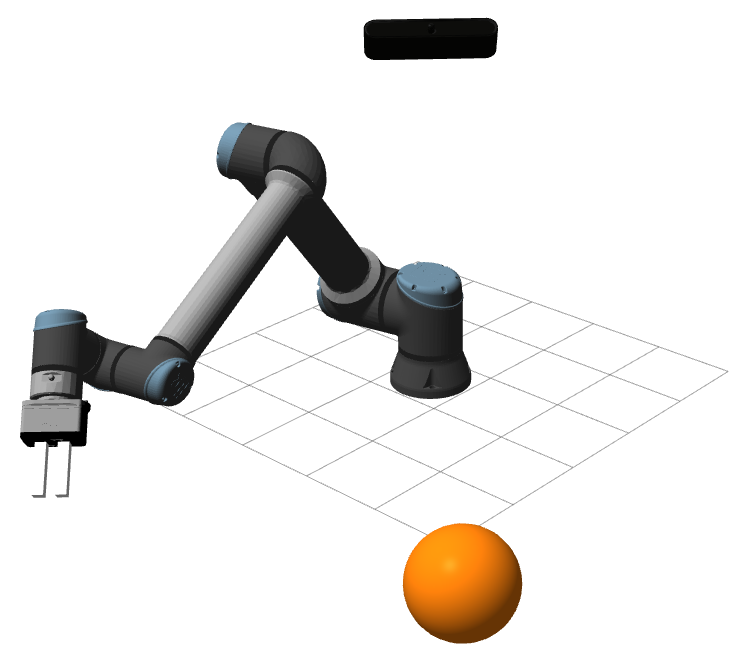
\includegraphics[width=.85\linewidth]{figs/chp6/traj_gazebo_obstacle.png}
    \end{subfigure}%
    \begin{subfigure}{.5\linewidth}
        \centering
        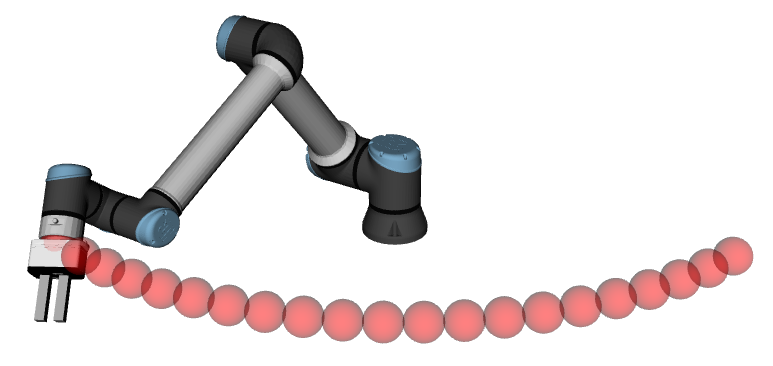
\includegraphics[width=\linewidth]{figs/chp6/traj_rviz.png}
    \end{subfigure}
    \caption{Simulation scenario with obstacle and offline generated trajectory}
    \label{fig:obstacle_test}
\end{figure}

\par Once the control service on the \ac{apf} controller is called with the \textit{play} instruction, the robot starts executing the trajectory. Since the obstacle node is not detecting any obstacles, the motion vector is equal to the attraction vector, therefore the executed trajectory is the same as the predefined one. When the robot approaches the obstacle, and the minimum distance constant is reached, a repulsion vector is generated making the final motion vector steer the robot away from the obstacle. Once the robot is enough distant from the obstacle and the repulsion vector disappears, it resumes the original trajectory. \autoref{fig:trajectory} shows this behavior, where the original and adjusted trajectories are plotted with the sphere obstacle.

\begin{figure}[h]
    \centering
    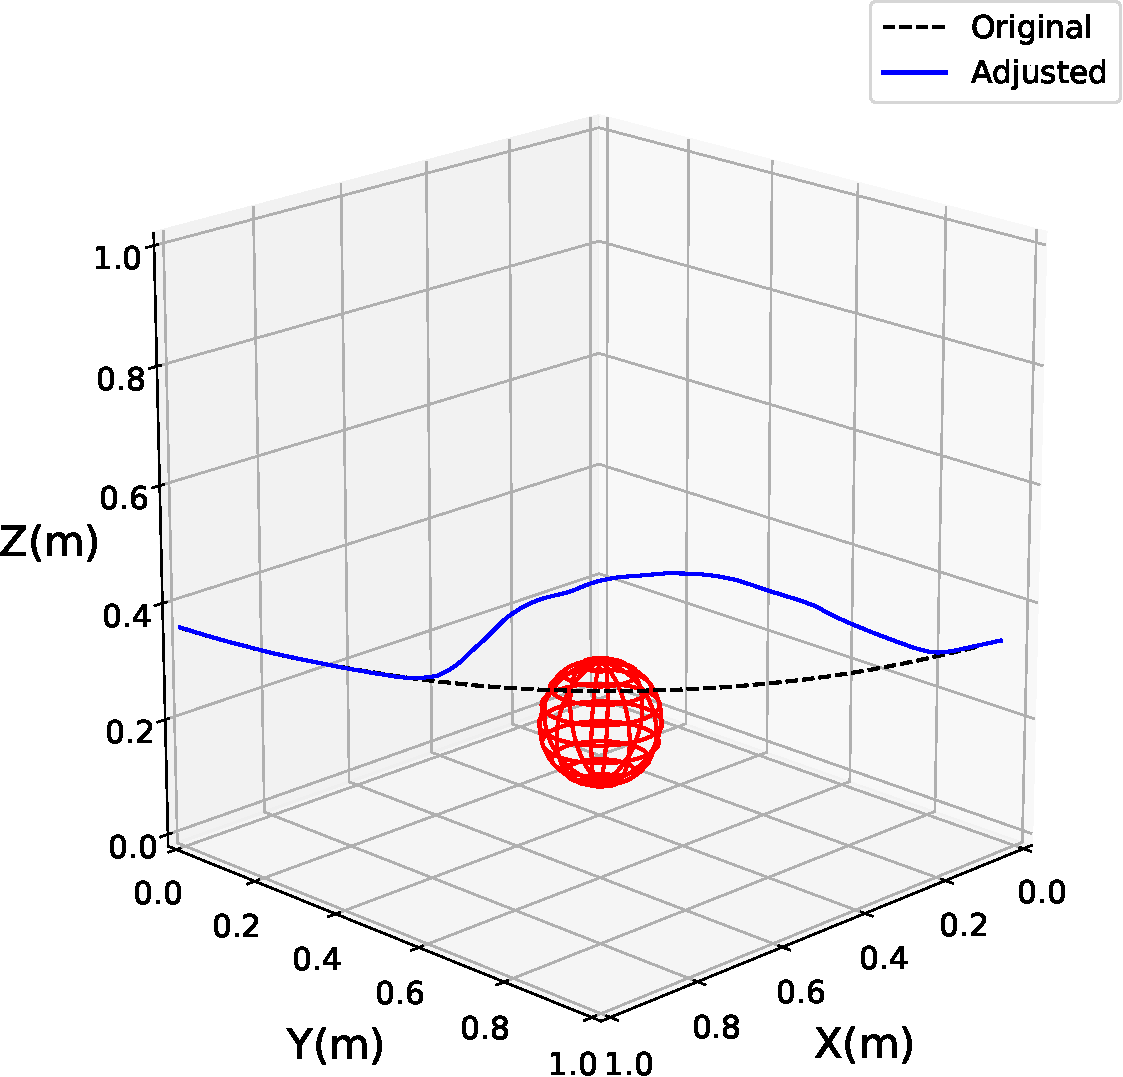
\includegraphics[width=0.6\linewidth]{figs/chp6/trajectory_3d.pdf}
    \caption{Execution of the trajectory with and without obstacle}
    \label{fig:trajectory}
\end{figure}

\par Having performed the base test with one obstacle, a set of tests with randomly placed and varying number of obstacles was performed in order to test the robustness of the collision avoidance architecture. The number of obstacles ranged from 0 to 5 and they were randomly placed in an area defined by the parameters in \autoref{tbl:random_obstacle}.

\begin{table}[h]
    \centering
    \begin{tabular}{|c|c|c|}
    \hline
    \textbf{Axis} & \textbf{Minimum} & \textbf{Maximum} \\ \hline
    \textbf{X} & 0.5 & 1.0 \\ \hline
    \textbf{Y} & 0.5 & 1.0 \\ \hline
    \textbf{Z} & 0.3 & 0.5 \\ \hline
    \end{tabular}
    \caption{Parameters for the random placement of obstacles}
    \label{tbl:random_obstacle}
\end{table}

\par Examples of the disposition of the randomly placed obstacles are shown in \autoref{fig:mult_obstacle_test}.

\begin{figure}[h]
    \centering
    \begin{subfigure}{.2\linewidth}
        \centering
        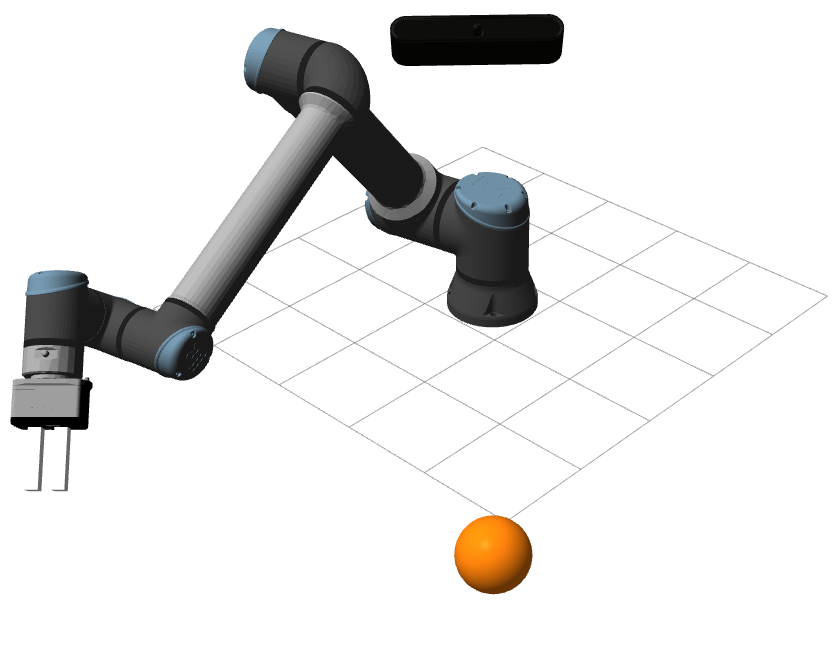
\includegraphics[width=.95\linewidth]{figs/chp6/obstacle_1.png}
    \end{subfigure}%
    \begin{subfigure}{.2\linewidth}
        \centering
        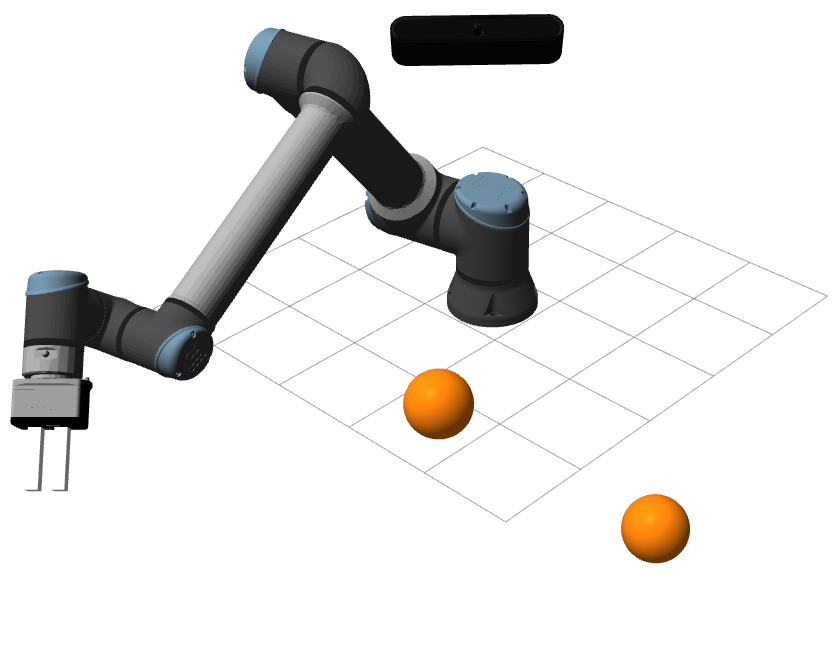
\includegraphics[width=.95\linewidth]{figs/chp6/obstacle_2.png}
    \end{subfigure}%
    \begin{subfigure}{.2\linewidth}
        \centering
        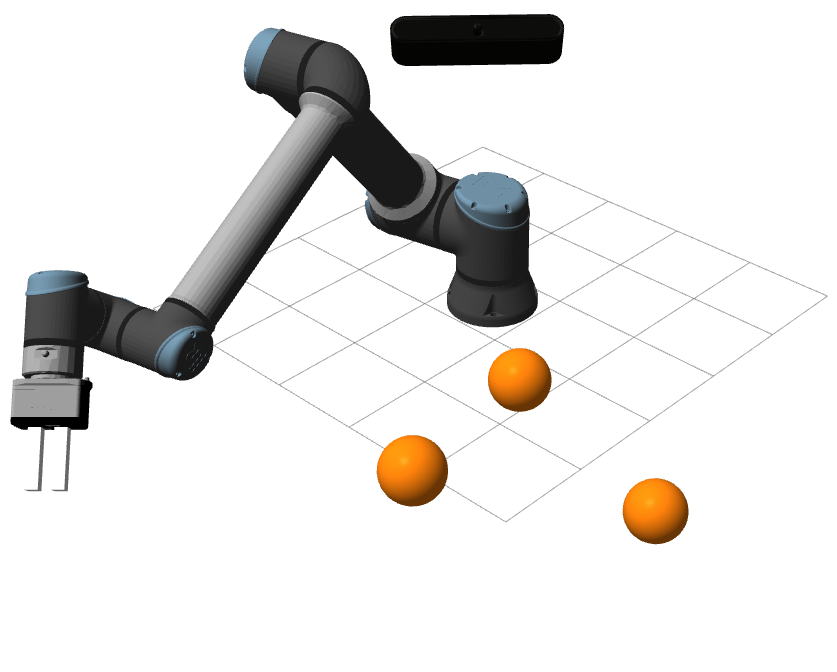
\includegraphics[width=.95\linewidth]{figs/chp6/obstacle_3.png}
    \end{subfigure}%
    \begin{subfigure}{.2\linewidth}
        \centering
        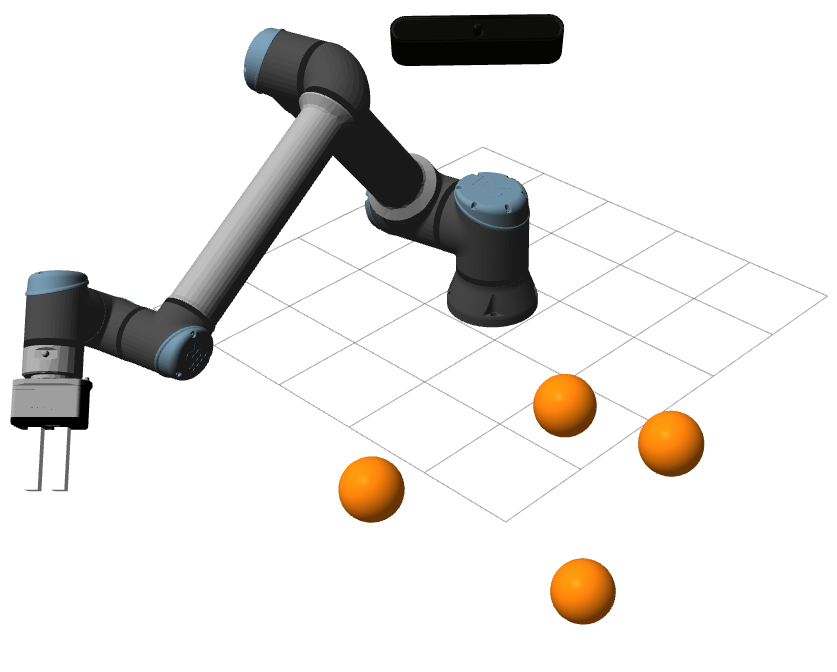
\includegraphics[width=.95\linewidth]{figs/chp6/obstacle_4.png}
    \end{subfigure}%
    \begin{subfigure}{.2\linewidth}
        \centering
        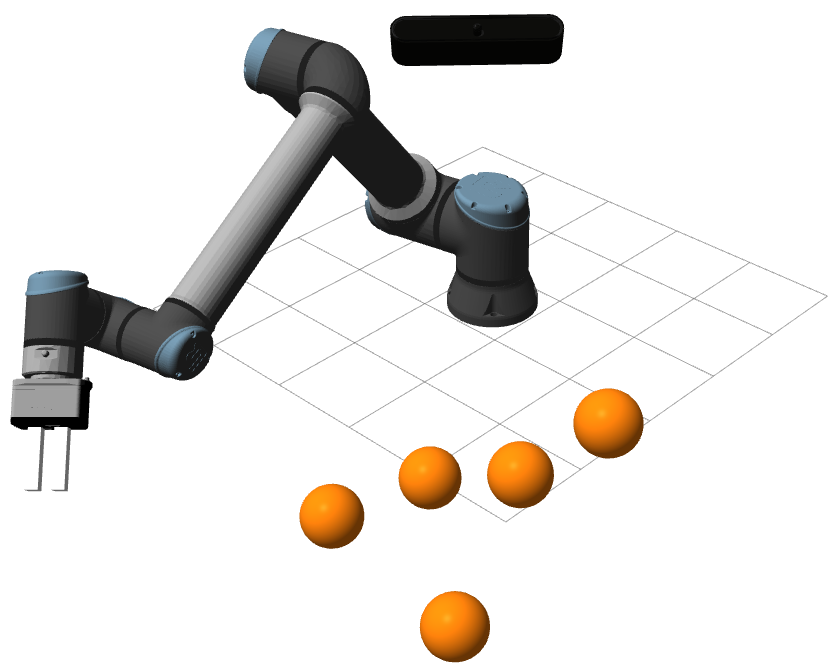
\includegraphics[width=.95\linewidth]{figs/chp6/obstacle_5.png}
    \end{subfigure}
    \caption{Simulation scenarios with multiple obstacles}
    \label{fig:mult_obstacle_test}
\end{figure}

\par The test consists on executing the trajectory of the previous test 10 times in each randomly generated environment. The ability to complete the trajectory without colliding with any obstacle, and the time it tool was recorded. These results are outlined in \autoref{tbl:random_obstacle_test}.

\begin{table}[h]
    \centering
    \begin{tabular}{|c|c|c|}
    \hline
    \textbf{Obstacles} & \textbf{Completed} & \textbf{Average Time} \\ \hline
    \textbf{0} & 10/10 & 11.43s \\ \hline
    \textbf{1} & 9/10 & 19.29s \\ \hline
    \textbf{2} & 7/10 & 20.44s \\ \hline
    \textbf{3} & 6/10 & 20.55s \\ \hline
    \textbf{4} & 2/10 & 22.32s \\ \hline
    \textbf{5} & 0/10 & --- \\ \hline
    \end{tabular}
    \caption{Results of the obstacle avoidance test}
    \label{tbl:random_obstacle_test}
\end{table}

\par The execution of the trajectory without obstacles in the environment is always successful, and the time is takes is proportional to the velocity configured in the robot controller. Once obstacles are introduced, the success rate decreases and the time it takes to reach the goal pose increases. For a reasonable amount of obstacles (1 or 2) the success rate is acceptable, but for an higher amount, the robot easily colides with obstacles and rarely completes the trajectory. This happens for a number of reasons:

\begin{itemize}
    \item The current implementation of the repulsion vector only takes into account one obstacle at a time, which is the closest, therefore, the repulsion caused by an obstacle can lead the robot to colide with another obstacle.
    \item Due to the previous fact, the robot can also get stuck between 2 obstacles that are equally distant from it, which despite not generating a collision, it will prevent the robot to reach its goal pose.
    \item The testing conditions are not realistic, and the placement of more than 3 obstacles in a small area such as the one previously described is an exaggeration created to test the limits of the architecture.
\end{itemize}


\par To solve this issues, the collision avoidance architecture should be improved by taking into account multiple obstacles simultaneously, and calculating their distance to multiple parts of the robot, and not just to the \ac{eef}. A possible solution to the local minimum problem, would be the replanning of the offline trajectory taking into account the obstacles identified. Due to the nature of the goals proposed for this Dissertation, these endeavours were not implemented but rather classified as future work.

% TODO Make a table with the response times of the obstacle detection (gazebo, from obstacle to movement)


\subsubsection{Real Environment}

\par Regarding the implementation of this task in a real scenario, the executed tests and recorded performance metrics were not the same as the simulation tests. Instead of testing the ability to adapt the trajectory in a cluttered environment, focus was given to the relation between robot speed and minimum collision distance. Reasons for this choice rely on the fact that arranging various obstacles in a real scenario is more time consuming than in the Gazebo simulator. On the other hand, the joint speed control in the simulator is not possible since, currently, the \ac{ur10e} Gazebo implementation only supports joint position based control. Therefore, since the \ac{ur10e} Polyscope interface allows velocity control through a speed slider variable, it is possible to correlate the speed of the robot \ac{eef} to the effectiveness of the collision avoidance architecture.

\par To achieve these metrics, a similar test was performed were a table served as a shared workspace, and the robot would execute a trajectory between its extremes. On the first test, there were no obstacles between the 2 points, but on the following tests an orange cone is placed in a position that would intentionally colide with the offline trajectory. \autoref{fig:col_real_test} illustrates both the execution of the trajectory without obstacles and with an orange cone directly interfering with the trajectory.

\begin{figure}[h]
    \centering
    \begin{subfigure}{.2\linewidth}
        \centering
        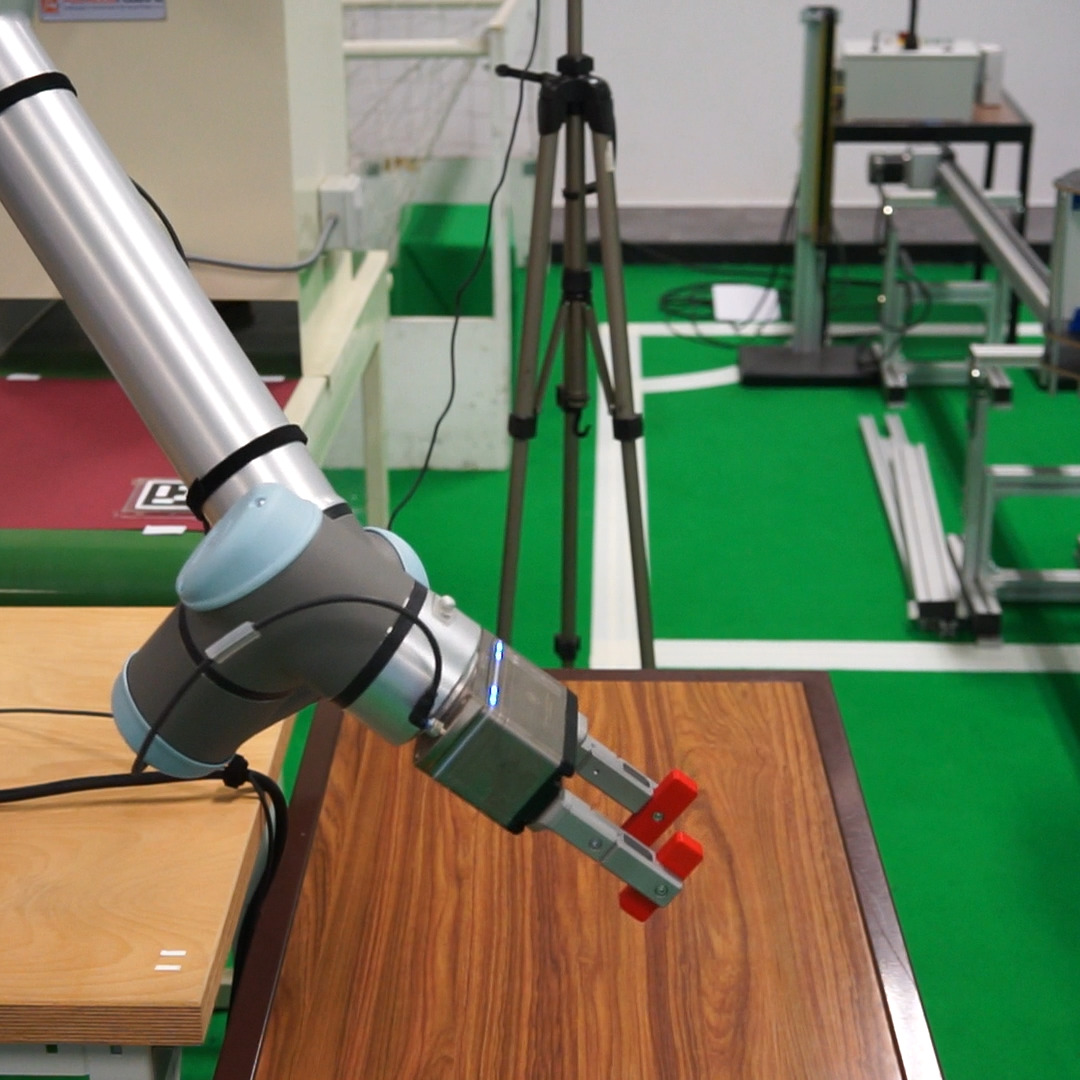
\includegraphics[width=.95\linewidth]{figs/chp6/col_real_no_1.jpg}
    \end{subfigure}%
    \begin{subfigure}{.2\linewidth}
        \centering
        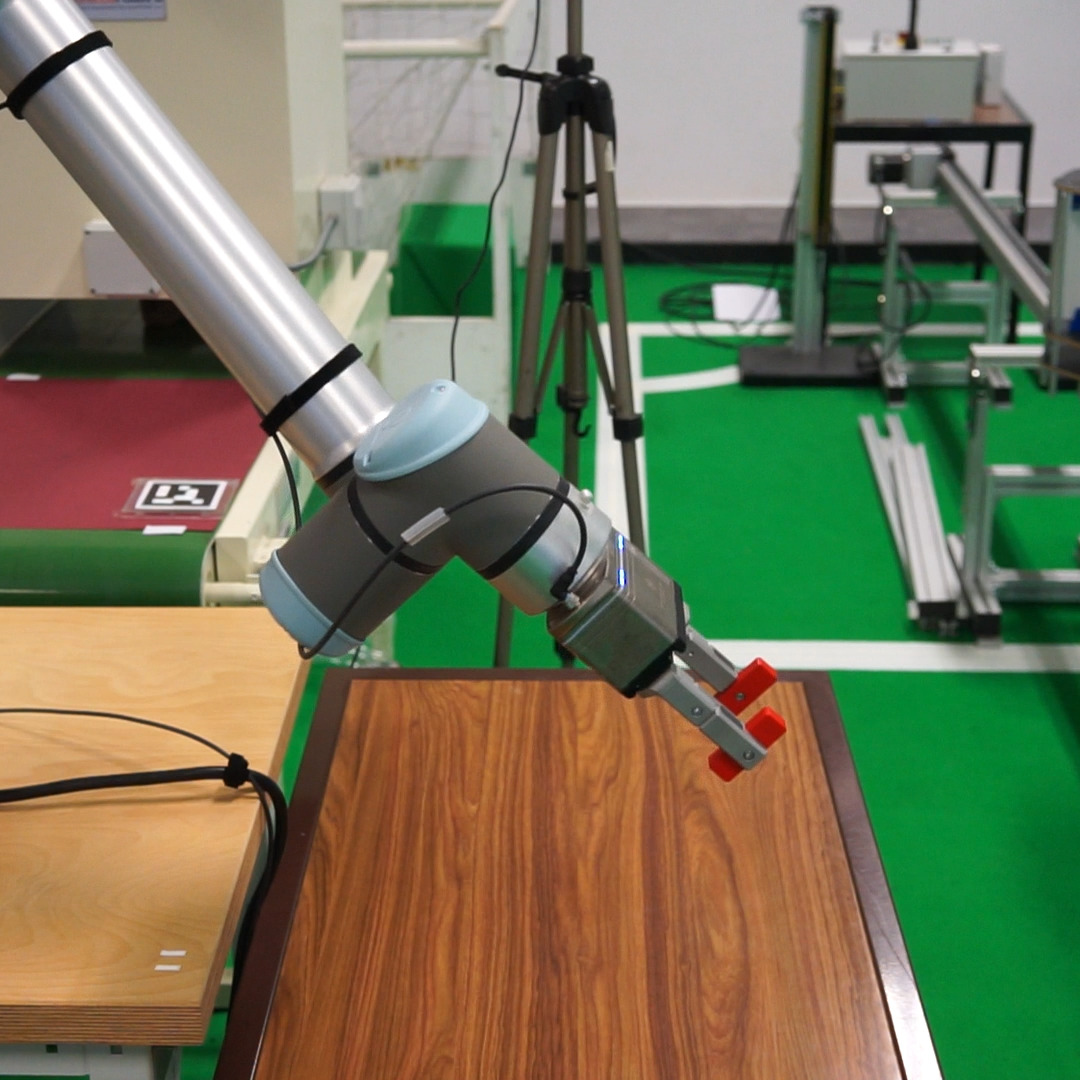
\includegraphics[width=.95\linewidth]{figs/chp6/col_real_no_2.jpg}
    \end{subfigure}%
    \begin{subfigure}{.2\linewidth}
        \centering
        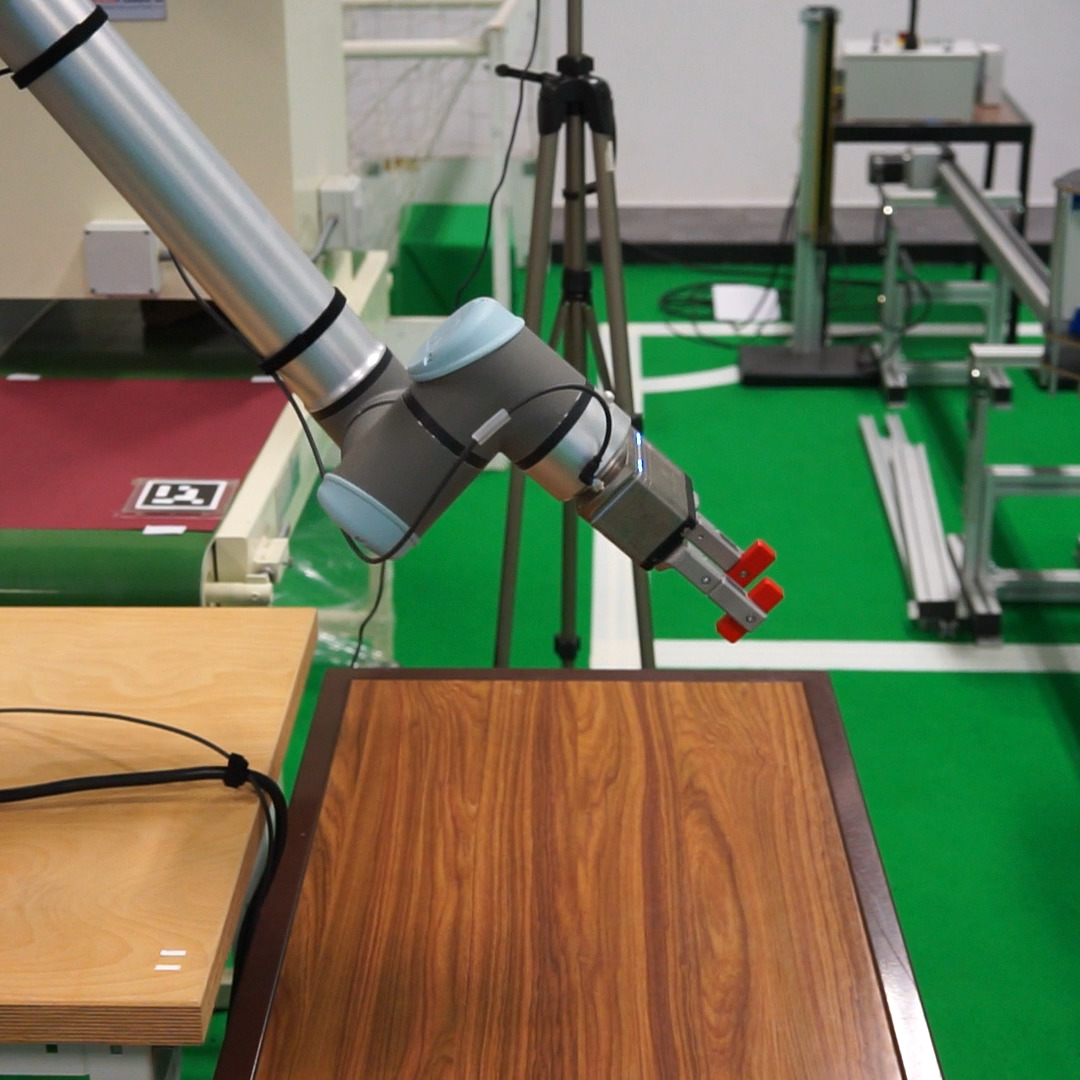
\includegraphics[width=.95\linewidth]{figs/chp6/col_real_no_3.jpg}
    \end{subfigure}%
    \begin{subfigure}{.2\linewidth}
        \centering
        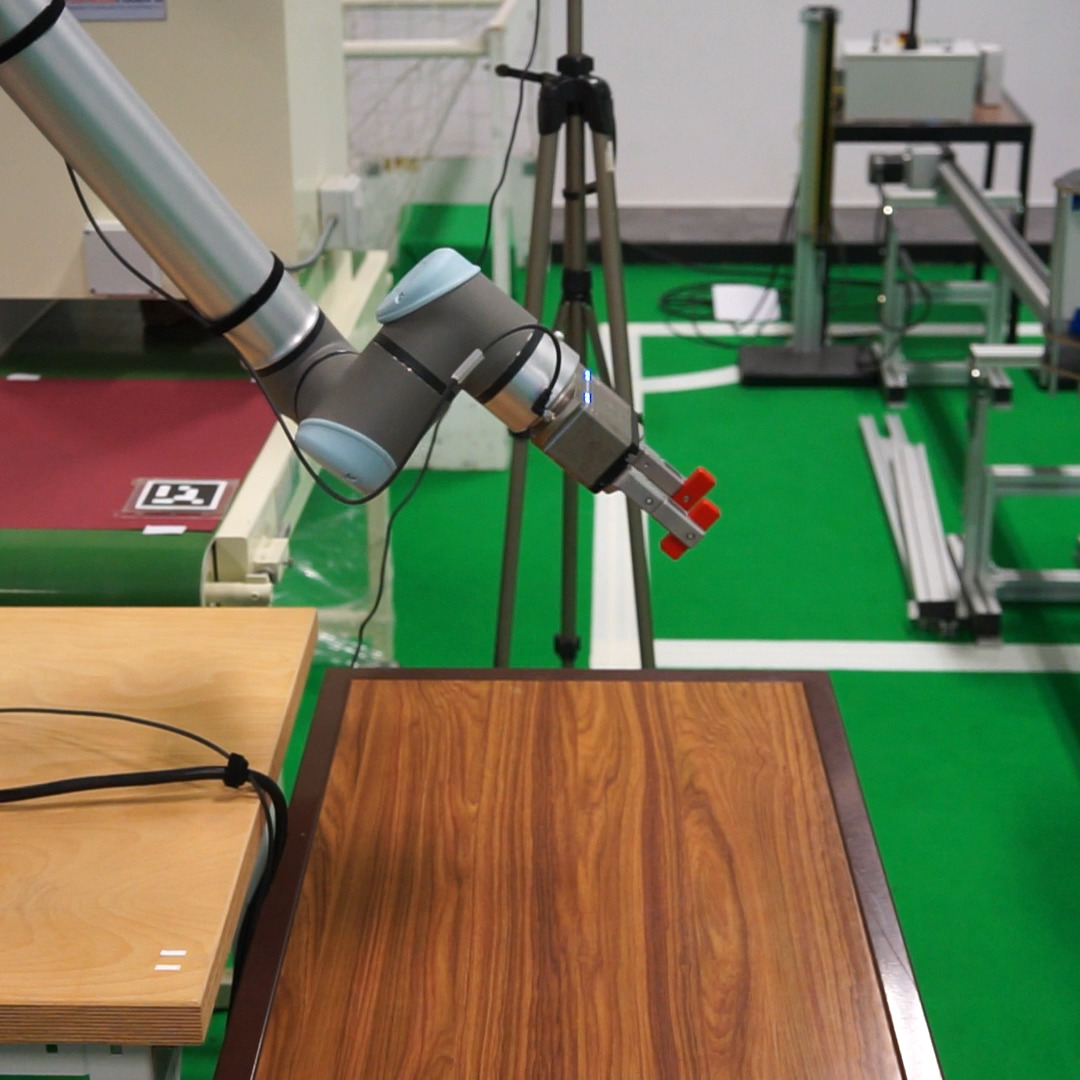
\includegraphics[width=.95\linewidth]{figs/chp6/col_real_no_4.jpg}
    \end{subfigure}%
    \begin{subfigure}{.2\linewidth}
        \centering
        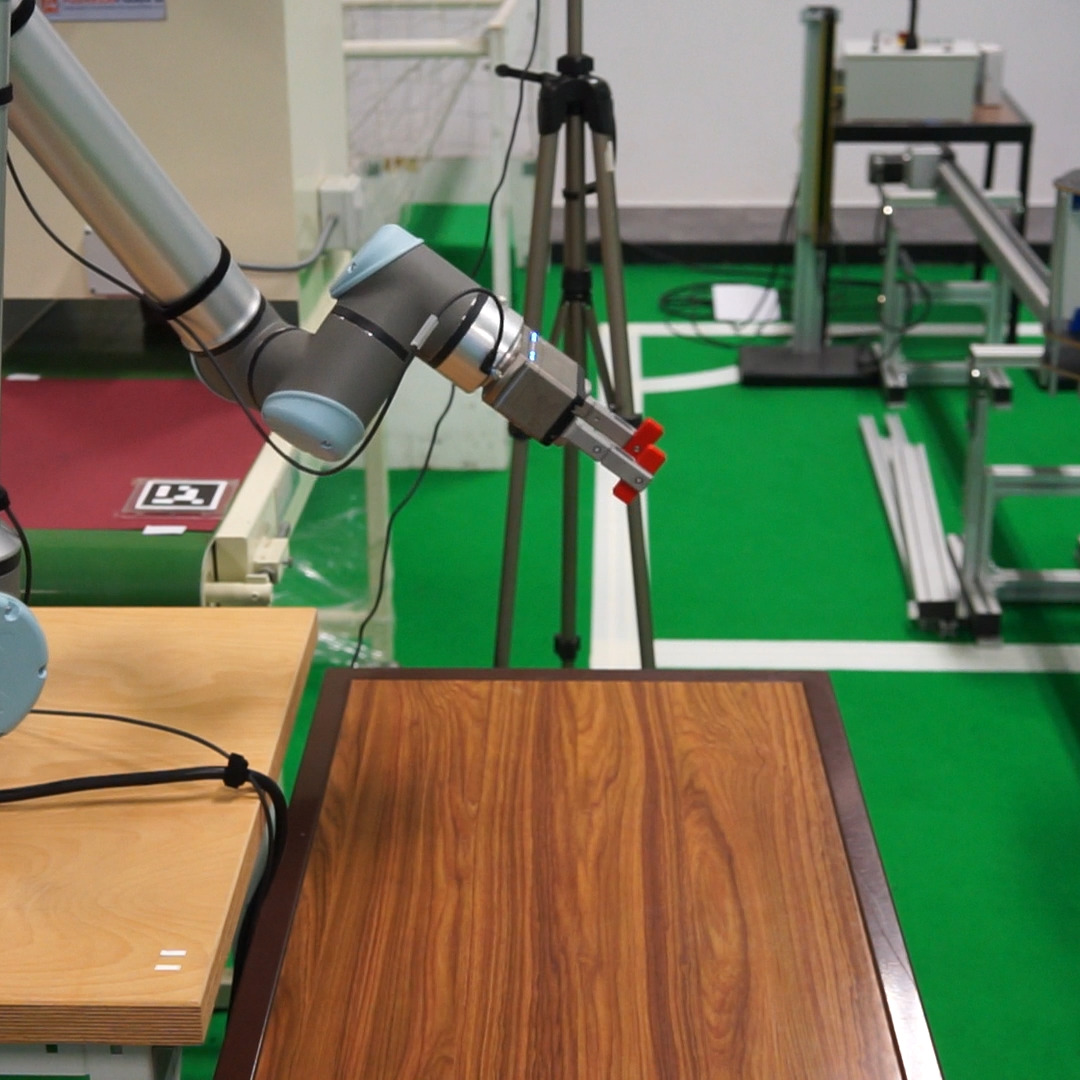
\includegraphics[width=.95\linewidth]{figs/chp6/col_real_no_5.jpg}
    \end{subfigure}
    \par\smallskip
    \begin{subfigure}{.2\linewidth}
        \centering
        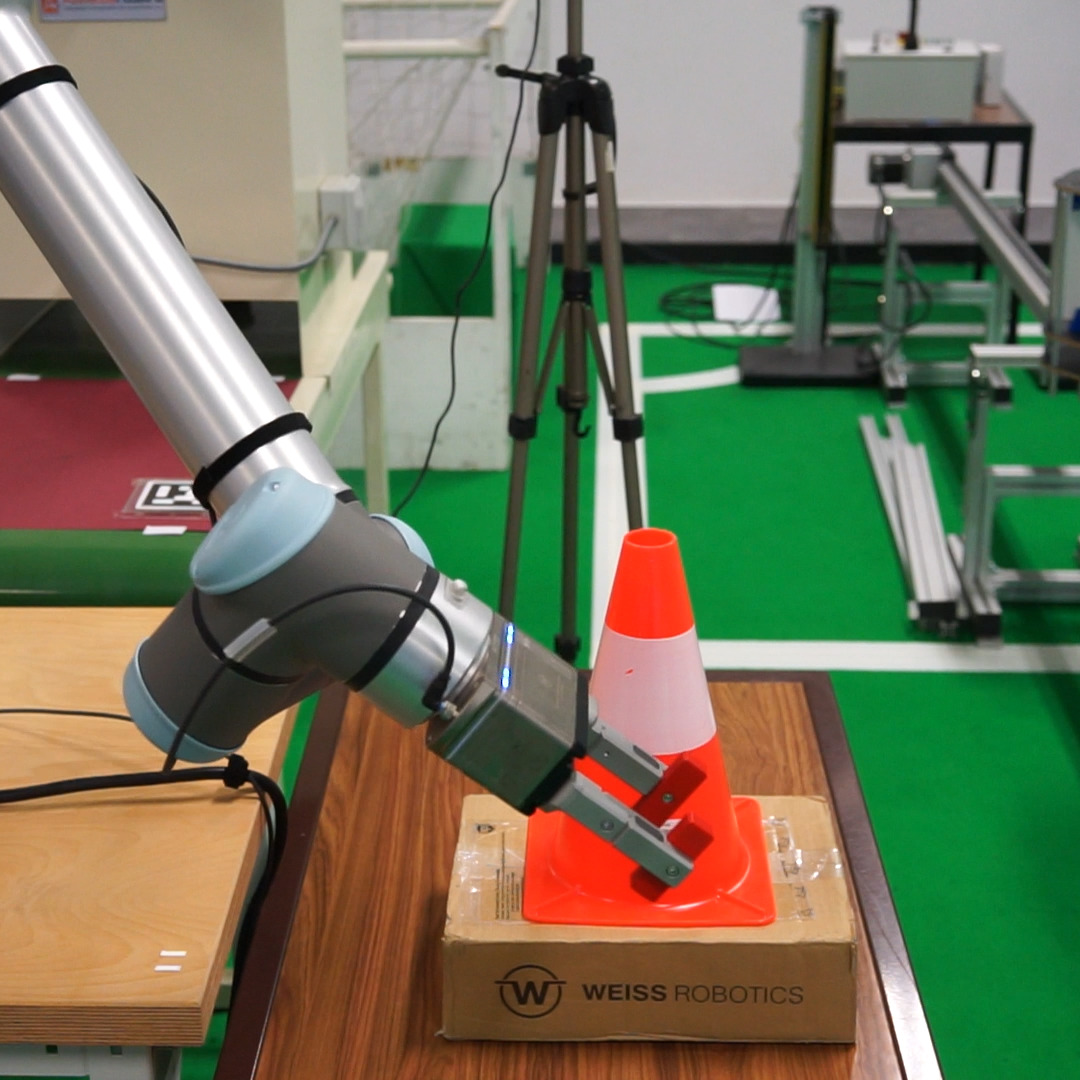
\includegraphics[width=.95\linewidth]{figs/chp6/col_real_1.jpg}
    \end{subfigure}%
    \begin{subfigure}{.2\linewidth}
        \centering
        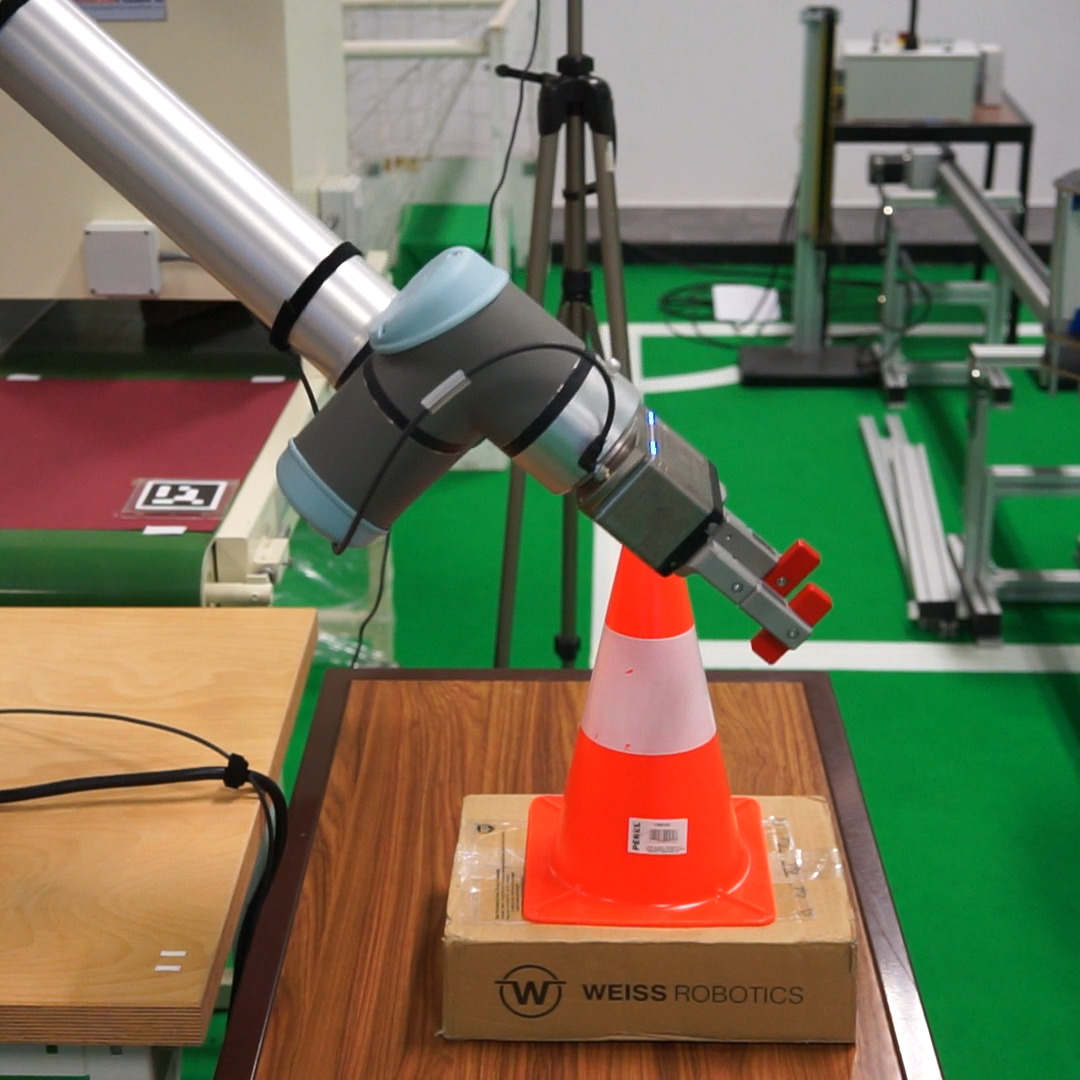
\includegraphics[width=.95\linewidth]{figs/chp6/col_real_2.jpg}
    \end{subfigure}%
    \begin{subfigure}{.2\linewidth}
        \centering
        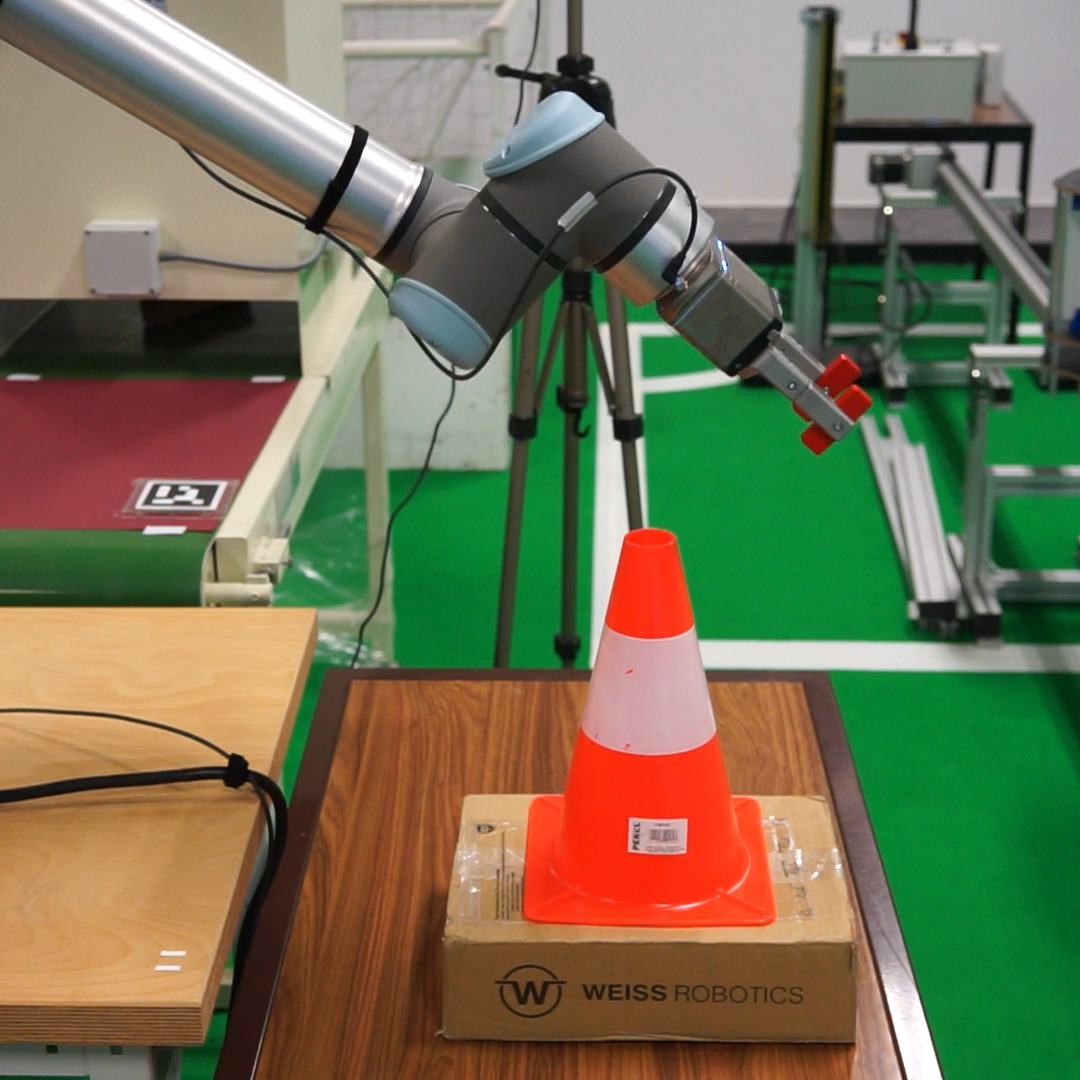
\includegraphics[width=.95\linewidth]{figs/chp6/col_real_3.jpg}
    \end{subfigure}%
    \begin{subfigure}{.2\linewidth}
        \centering
        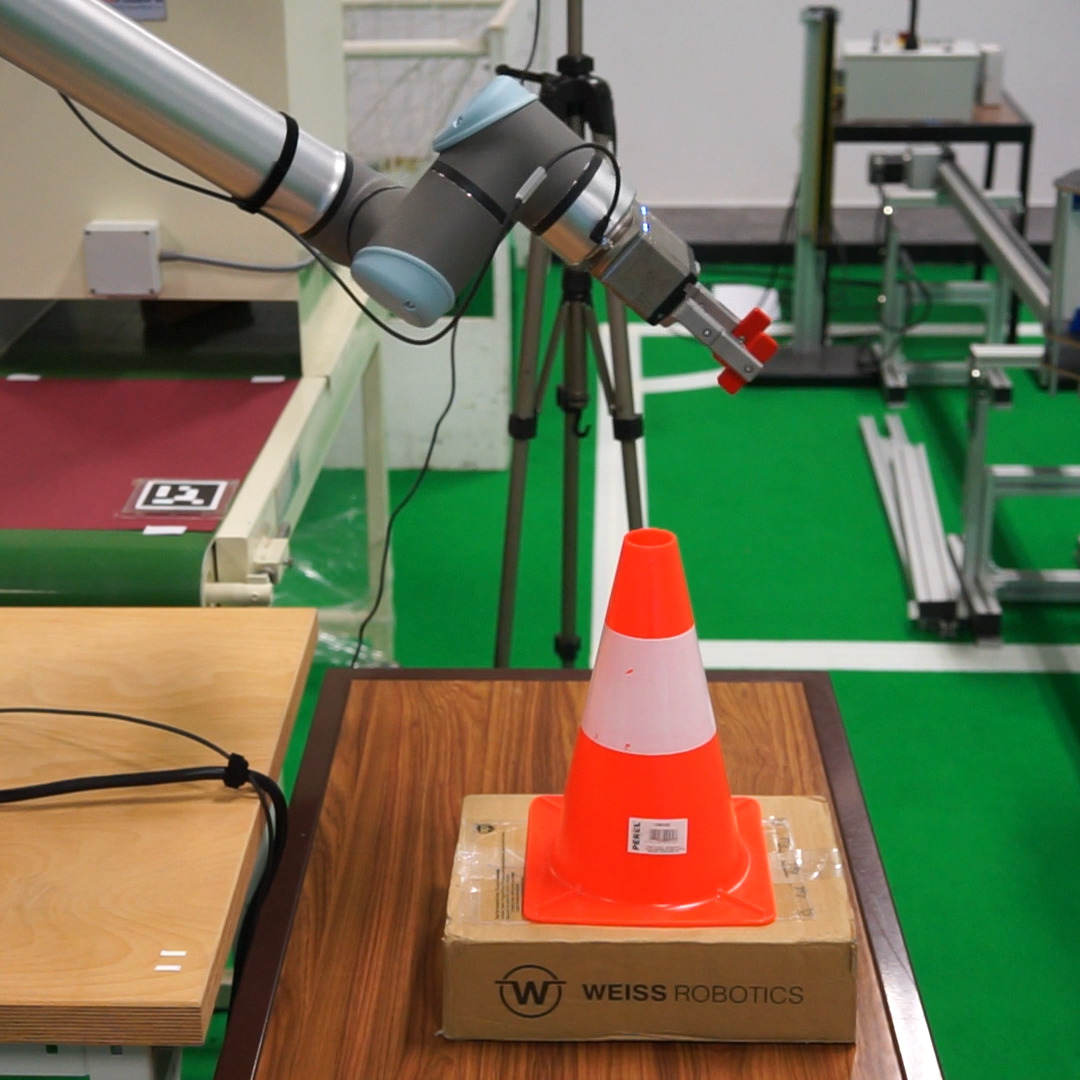
\includegraphics[width=.95\linewidth]{figs/chp6/col_real_4.jpg}
    \end{subfigure}%
    \begin{subfigure}{.2\linewidth}
        \centering
        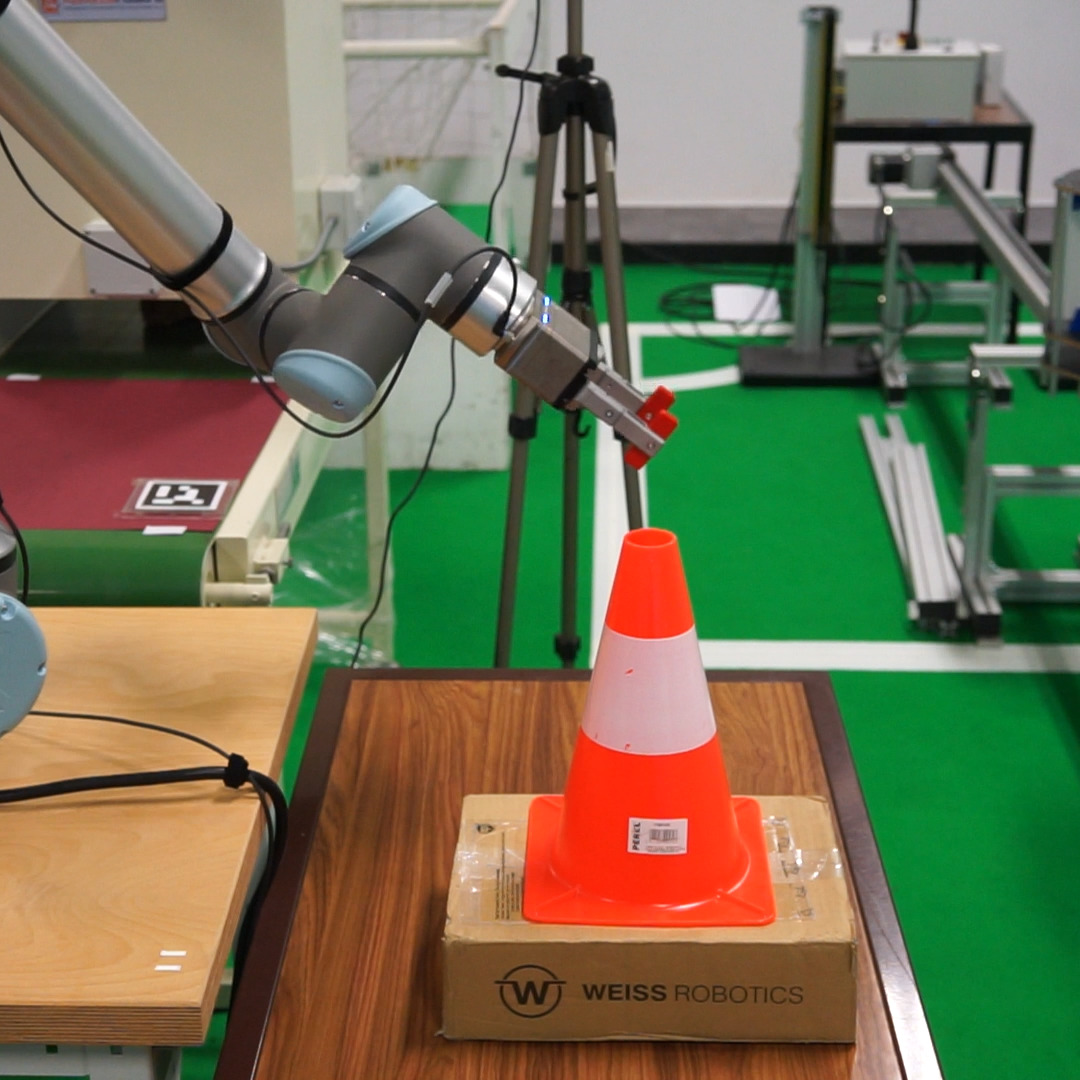
\includegraphics[width=.95\linewidth]{figs/chp6/col_real_5.jpg}
    \end{subfigure}
    \caption{Succession of steps of the collision avoidance test}
    \label{fig:col_real_test}
\end{figure}

\par As observed, the robot is able to avoid the obstacle, complete its trajectory and keep a safe distance from the obstacle, preventing a collision with any part of the robot. This base test was performed with a speed slider of 10\%. To observe how the robot speed impacts its behavior when avoiding obstacles, this test was repeated in multiple speed slider settings. \autoref{fig:real_col_speed} demonstrates the trajectory of the \ac{eef} when performing the aforementioned tests, and it also denotes in space the points that were identified as obstacles.

\begin{figure}[h]
    \centering
    \begin{subfigure}{.5\linewidth}
        \centering
        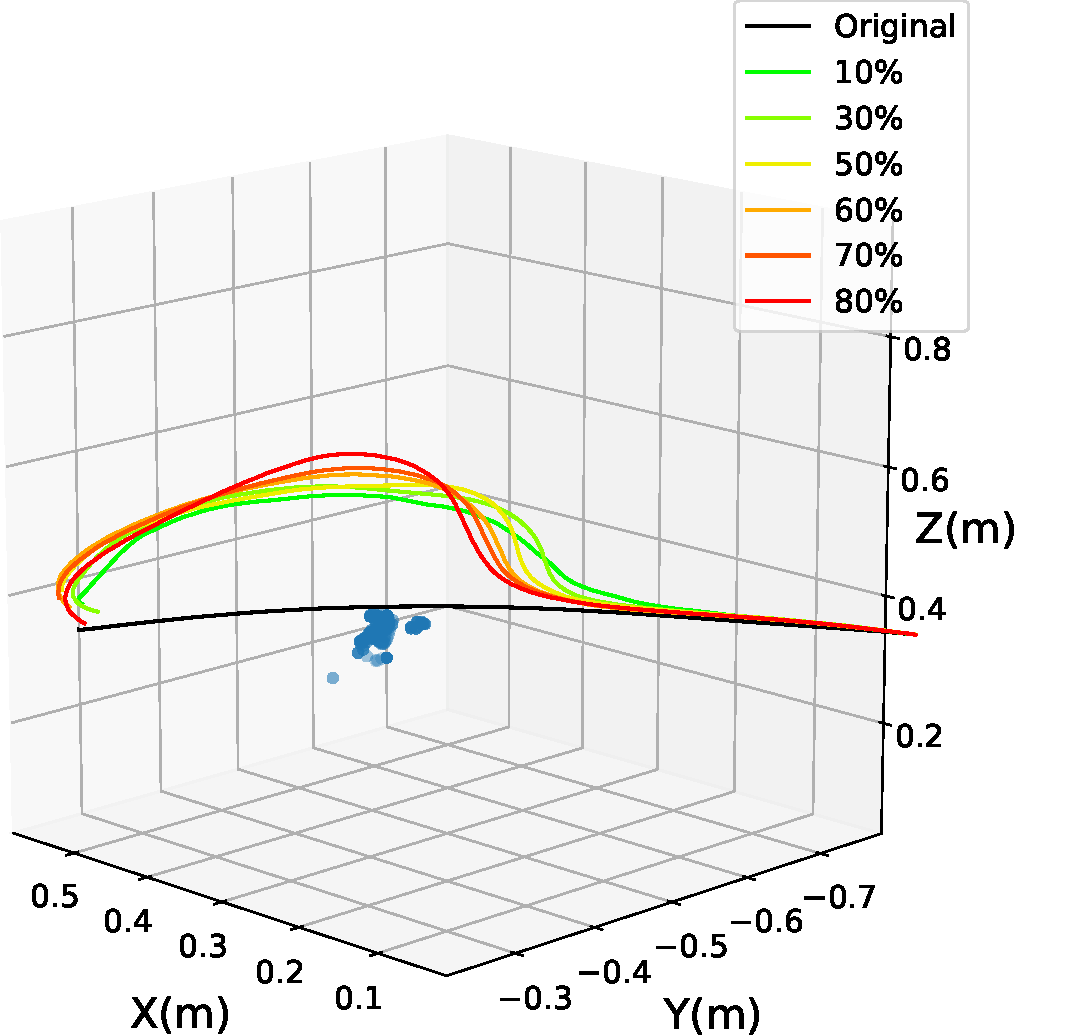
\includegraphics[width=.95\linewidth]{figs/chp6/traj_obstacles_1.pdf}
    \end{subfigure}%
    \begin{subfigure}{.5\linewidth}
        \centering
        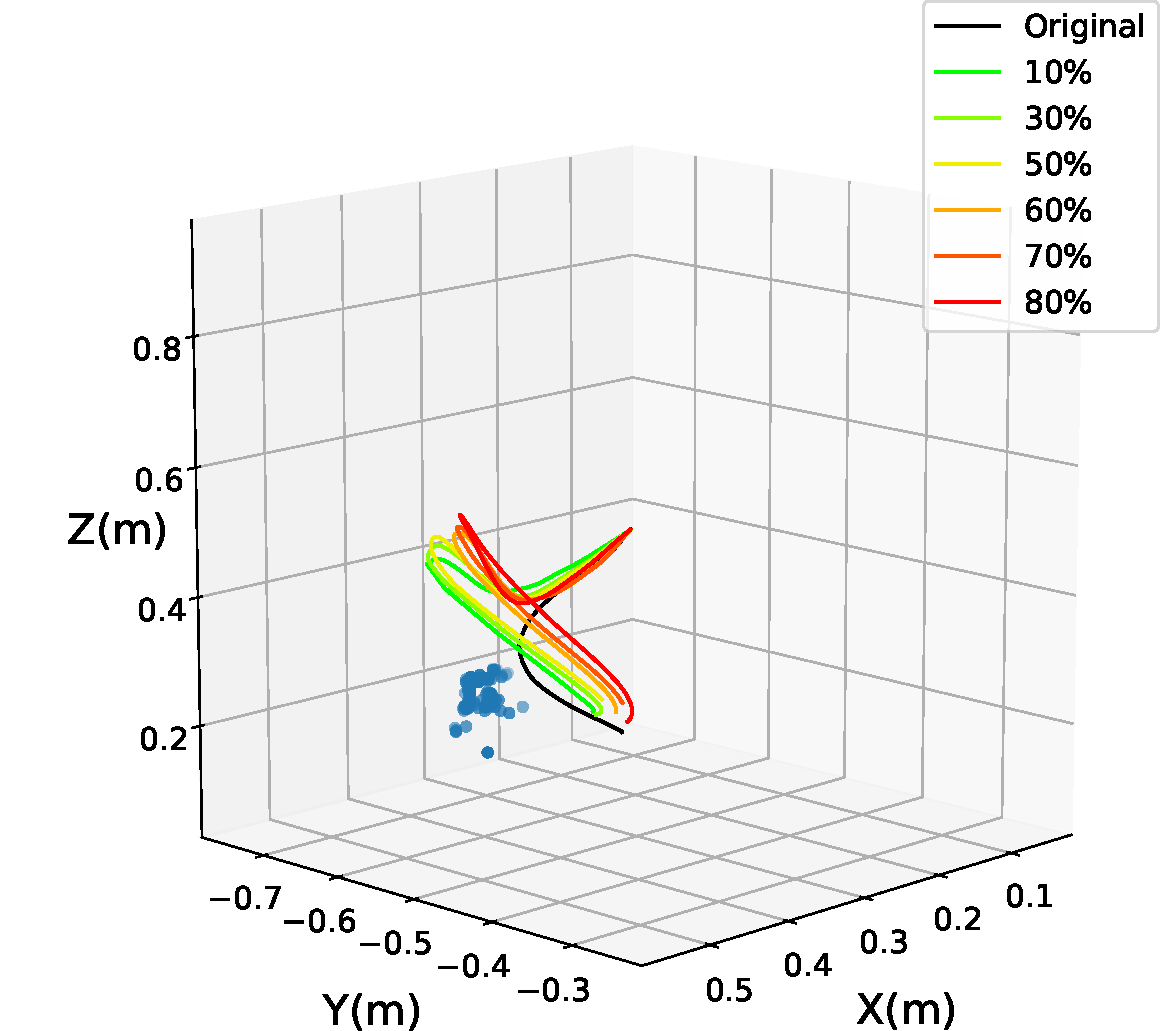
\includegraphics[width=.95\linewidth]{figs/chp6/traj_obstacles_2.pdf}
    \end{subfigure}
    \caption{Collision avoidance in real scenario with multiple speed settings}
    \label{fig:real_col_speed}
\end{figure}

\par When increasing the speed of the robot, the point in space where the robot starts adapting its trajectory gets closer to the identified obstacles. The maximum speed slider value was 80\% due to the fact that an higher values causes a collision. \autoref{tbl:speed_dist} shows in each speed setting the minimum distance that the robot \ac{eef} was in relation to the identified obstacle at that time. The table also shows the conversion of speed slider to real \ac{eef} speed in $m/s$.

\begin{table}[h]
    \centering
    \begin{tabular}{|c|c|c|}
    \hline
    \textbf{Speed Slider} & \textbf{EEF Speed} & \textbf{Minimum Distance} \\ \hline
    \textbf{0.1}          & 0.054              & 0.21749                   \\ \hline
    \textbf{0.3}          & 0.155              & 0.21157                   \\ \hline
    \textbf{0.5}          & 0.234              & 0.19893                   \\ \hline
    \textbf{0.6}          & 0.282              & 0.19460                   \\ \hline
    \textbf{0.7}          & 0.316              & 0.19105                   \\ \hline
    \textbf{0.8}          & 0.359              & 0.18347                   \\ \hline
    \textbf{0.9}          & 0.406              & Collision                 \\ \hline
    \textbf{1.0}          & 0,449              & Collision                 \\ \hline
    \end{tabular}
    \caption{Minimum EEF distance to obstacle relative to its speed}
    \label{tbl:speed_dist}
\end{table}

\par The configured parameter, on the collision avoidance architecture, by which a point is considered to be inside the \ac{roi}, for the execution of theses tests, was 0.3m. The results obtained are as expected since when the robot moves with a relatively low speed, the distance it keeps from the obstacle is constant and high enough to prevent collisions, throughout the execution of the trajectory. But as the speed of the robot increases, the minimum distance starts to decrease, reaching a point where this implementation is not fast enough to make the robot avoid the obstacle. This behavior happens for a couple of reasons:

\begin{itemize}
    \item The distance between the \ac{eef} and the tip of the gripper tool is exactly 0.18m, therefore, according to \autoref{tbl:speed_dist}, when the speed slider is higher than 80\%, the robot colides with the obstacle because it cannot maintain a minimum distance higher than 0.18m.
    \item The rate of identification of obstacles is limited, due to the fact that the Microsoft Kinect camera can only publish point clouds at a maximum rate of 30Hz. The fact that this architecture and tests were executed on a laptop also does not help performance.
    \item As demonstrated in \autoref{chp:4-obstacle}, when identifying obstacles and calculating the repulsion vector, only the \ac{eef} position is used.
\end{itemize}

\par A simple fix to obtain better results in this test is increasing the \ac{roi} minimum distance constant, but in theory, 0.3m should be enough to avoid collisions at the \ac{eef} level, therefore, the performance of the robot when avoiding obstacles can be improved in various other aspects. The collision avoidance architecture should use more points to identify obstacles and calculate the repulsion vector, than using only the \ac{eef} position. Examples are the tip of the gripper tool and the wrist links. The use of a faster camera with an higher sample frequency should also be considered, since, by industry standards, 30Hz is not enough to detect dynamic obstacles. Even though the results can be improved with the aforementioned solutions, this implementation is considered successful in what it proposes, which is the execution of an offline trajectory with realtime dynamic collision avoidance.


% TODO Explain that this tests are giving more focus to the algorithms implemented and not on the tasks itself, because the tasks are all able to be completed... The more important aspect is the capabilities of the implemented algorithms (payload compensation, collision avoidance)

\section{System Stability}

% TODO Make tests on system latency and performance (in all components)

% System cannot maintain activity for long periods of time
\par A more general performance metric is the ability for the system to maintain activity for long periods of time. There are several factors that prevent this from happen. During the execution of the previous tests and any other time directly interfacing with the robot, there were some events that injured the overall experience.

% Driver loses connection
\par For instance, at random instances, when the robot had been correctly functioning for a certain amount of time, e.g. 20 minutes, the system will lose connection with the robot. More specifically, the \ac{ur} \ac{ros} driver looses connection to the \ac{rtde} interface, or in some instances, the client program that is running on the robot, requesting commands to the driver suddenly stops its execution. The cause of this problem was not studied since there was no observable pattern on the instances that is happened. The solution was to call the \textbackslash\textit{resend\_robot\_program} \ac{ros} service made available by the driver and the connection would resume.

% Robot makes protective stops based when large amounts of force are applied
\par Another example is the fact that, because we are dealing with a cobot and the joints are force sensitive, when applying large amounts of force on the \ac{eef}, the cobot will make a protective stop, giving the user a violation alert, explaining that a force or speed limit was exceeded. Other examples of protective stops are prone to happen when the user couples high amounts of weight to the \ac{eef}. This happens because this weight is not reported to the \ac{ur10e} Polyscope interface. It is obvious that the \ac{ur10e} internal controllers need to know the correct value of payload in order to correctly calculate the necessary torques to apply in each joint, but as was explained in \autoref{ssec:ft_internal_comp}, not reporting the payload parameters to the \ac{ur10e} internal system is a necessary tradeoff for obtaining cohesive \ac{ft} measurements on the \ac{eef}.

% Tests were implemented on laptop
\par A final remark on system performance gives light to the fact that all components of this system were tested and implemented on a laptop with an Intel Core i7-8550U and 16Gb of \acs{ram}. 